\documentclass[11pt,a4paper]{article}

% Pacchetti fondamentali
\usepackage[utf8]{inputenc}
\usepackage[italian]{babel}
\usepackage{amsmath}
\usepackage{graphicx}
\usepackage{geometry}
\usepackage{booktabs}
\usepackage{float}
\usepackage{hyperref}
\usepackage{caption}
\usepackage{longtable}
\usepackage{booktabs}
\usepackage{multirow}

% Margini del testo ripristinati a 2.5cm (standard accademico)
\geometry{a4paper, top=2.5cm, bottom=2.5cm, left=2.5cm, right=2.5cm}

\title{\textbf{Analisi delle Prestazioni di Modelli Centralizzati ILP per il Task Routing al variare della Deadline}}
\author{Claudio Bagini 2045337}
\date{\today}

\begin{document}

\maketitle

\section{Introduzione}
Nel contesto dei sistemi distribuiti moderni e dell'edge computing, l'allocazione efficiente delle risorse computazionali (Resource Allocation) e l'istradamento dei task (Task Routing) rappresentano sfide critiche e di primaria importanza. 

Il sistema analizzato in questo studio sfrutta un approccio centralizzato basato su Integer Linear Programming (ILP) per mappare le richieste in ingresso sui nodi server disponibili. A differenza delle euristiche, che compiono scelte ottime a livello puramente locale (ma spesso sub-ottime a livello globale), il modello ILP garantisce l'individuazione di una soluzione matematicamente perfetta per un dato set di richieste.

Per comprendere a fondo l'impatto delle policy di orchestrazione e il comportamento del solutore centralizzato sotto stress, il modello è stato testato imponendo due diverse strategie di mappatura (\textit{Objective Mapping}) nella funzione obiettivo:
\begin{itemize}
    \item \textbf{Mapping Time:} I pesi della funzione obiettivo privilegiano la minimizzazione del tempo totale di risposta e di trasmissione ($W_{lat}=1, W_{en}=0$). Questa strategia è cruciale per i servizi altamente sensibili al ritardo (delay-sensitive).
    \item \textbf{Mapping Energy:} I pesi della funzione obiettivo privilegiano il risparmio energetico dei nodi e della rete ($W_{lat}=0, W_{en}=1$), parametro fondamentale per estendere la vita operativa di infrastrutture con rigidi vincoli di power-budget.
\end{itemize}
Le simulazioni mirano a individuare i colli di bottiglia fisici e logici del sistema e a valutare quali configurazioni di \textit{Batch Size} (dimensione della coda di richieste aggregata) e \textit{Batch Timeout} (tempo massimo di attesa prima di innescare l'ILP) garantiscano la maggiore resilienza al variare del tasso di arrivo delle richieste nella rete.

\section{Setup Sperimentale}
Le simulazioni sono state eseguite mantenendo un set di parametri di base costanti (ispirati al paper ICDCS di riferimento), al fine di isolare l'impatto delle metriche di interesse.

\subsection{Parametri e Variabili dell'Esperimento}
\begin{itemize}
    \item \textbf{Budget Energetico Globale:} Fissato rigorosamente a 80 KJ per l'intera durata di ogni iterazione di simulazione.
    \item \textbf{Arrival Rate (Carico di Rete):} Variabile indipendente principale. Il tasso di arrivo delle richieste è stato modulato per simulare scenari di traffico progressivo: da 2, 3, 4, 6, 8 fino a 10 richieste al secondo. Nel motore del simulatore, questi valori corrispondono a tempi di inter-arrivo (\textit{AT}) decrescenti (da $0.5$ a $0.1$ secondi).
    \item \textbf{Configurazioni di Batching:} Per ogni livello di \textit{Arrival Rate}, sono state testate molteplici configurazioni incrociate. Variando la \textit{Batch Size} (BS), si è stabilito quante richieste accumulare prima di avviare il solutore ILP (da 1 a 20). Variando il \textit{Batch Timeout} (BT), si è imposto un limite temporale massimo per prevenire lo stallo delle richieste (starvation) in scenari di traffico rado.
    \item \textbf{Coefficienti di Ponderazione ($\alpha$, $\beta$, $\gamma$):} In stretta conformità con il modello matematico del paper di riferimento, i vettori dei pesi che regolano i trade-off e i costi delle risorse all'interno della formulazione ILP sono stati mantenuti costanti, garantendo la coerenza dell'esperimento. Nello specifico, i parametri di profilazione sono stati fissati ai seguenti valori vettoriali: $\alpha = (0.3, 0.5, 0.2)$, $\beta = (0.4, 0.35, 0.25)$ e $\gamma = (0.7, 0.3)$.
    \item \textbf{Rilassamento della Deadline:} In questa serie di esperimenti, il vincolo temporale imposto sui task è stato progressivamente allentato, testando un delta incrementale del 10\%, 20\% e 30\% rispetto al valore di base.
\end{itemize}

\section{Migliorie e Correzioni Apportate}
In questa sezione vengono illustrate sinteticamente le principali modifiche apportate al simulatore. 

\begin{itemize}
    \item \textbf{Modifica della formula per il calcolo della deadline:} È stata introdotta una differenziazione logica nel calcolo della deadline assegnata ai task per tenere conto della latenza di raggruppamento. La nuova formulazione del vincolo temporale $D_r$ è così definita:
    \begin{equation}
        D_r = 
        \begin{cases} 
        (1.0 + \Delta_D) \cdot \left( d_{cpu} + d_{net} + d_{down} + \frac{1}{2} T_{batch} \right) & \text{con orchestratore} \\
        (1.0 + \Delta_D) \cdot \left( d_{cpu} + d_{net} + d_{down} \right) & \text{senza orchestratore}
        \end{cases}
    \end{equation}
    dove $\Delta_D$ rappresenta l'incremento percentuale tollerato, mentre $T_{batch}$ indica il parametro di \texttt{centralized\_batch\_timeout}. Questa correzione assicura che il tempo trascorso in attesa della risoluzione del routing non consumi in modo sproporzionato il margine temporale utile del task.
\end{itemize}


\section{Configurazione Energy}

    \subsection{Success Rate}

        \begin{figure}[H]
        \makebox[\textwidth][c]{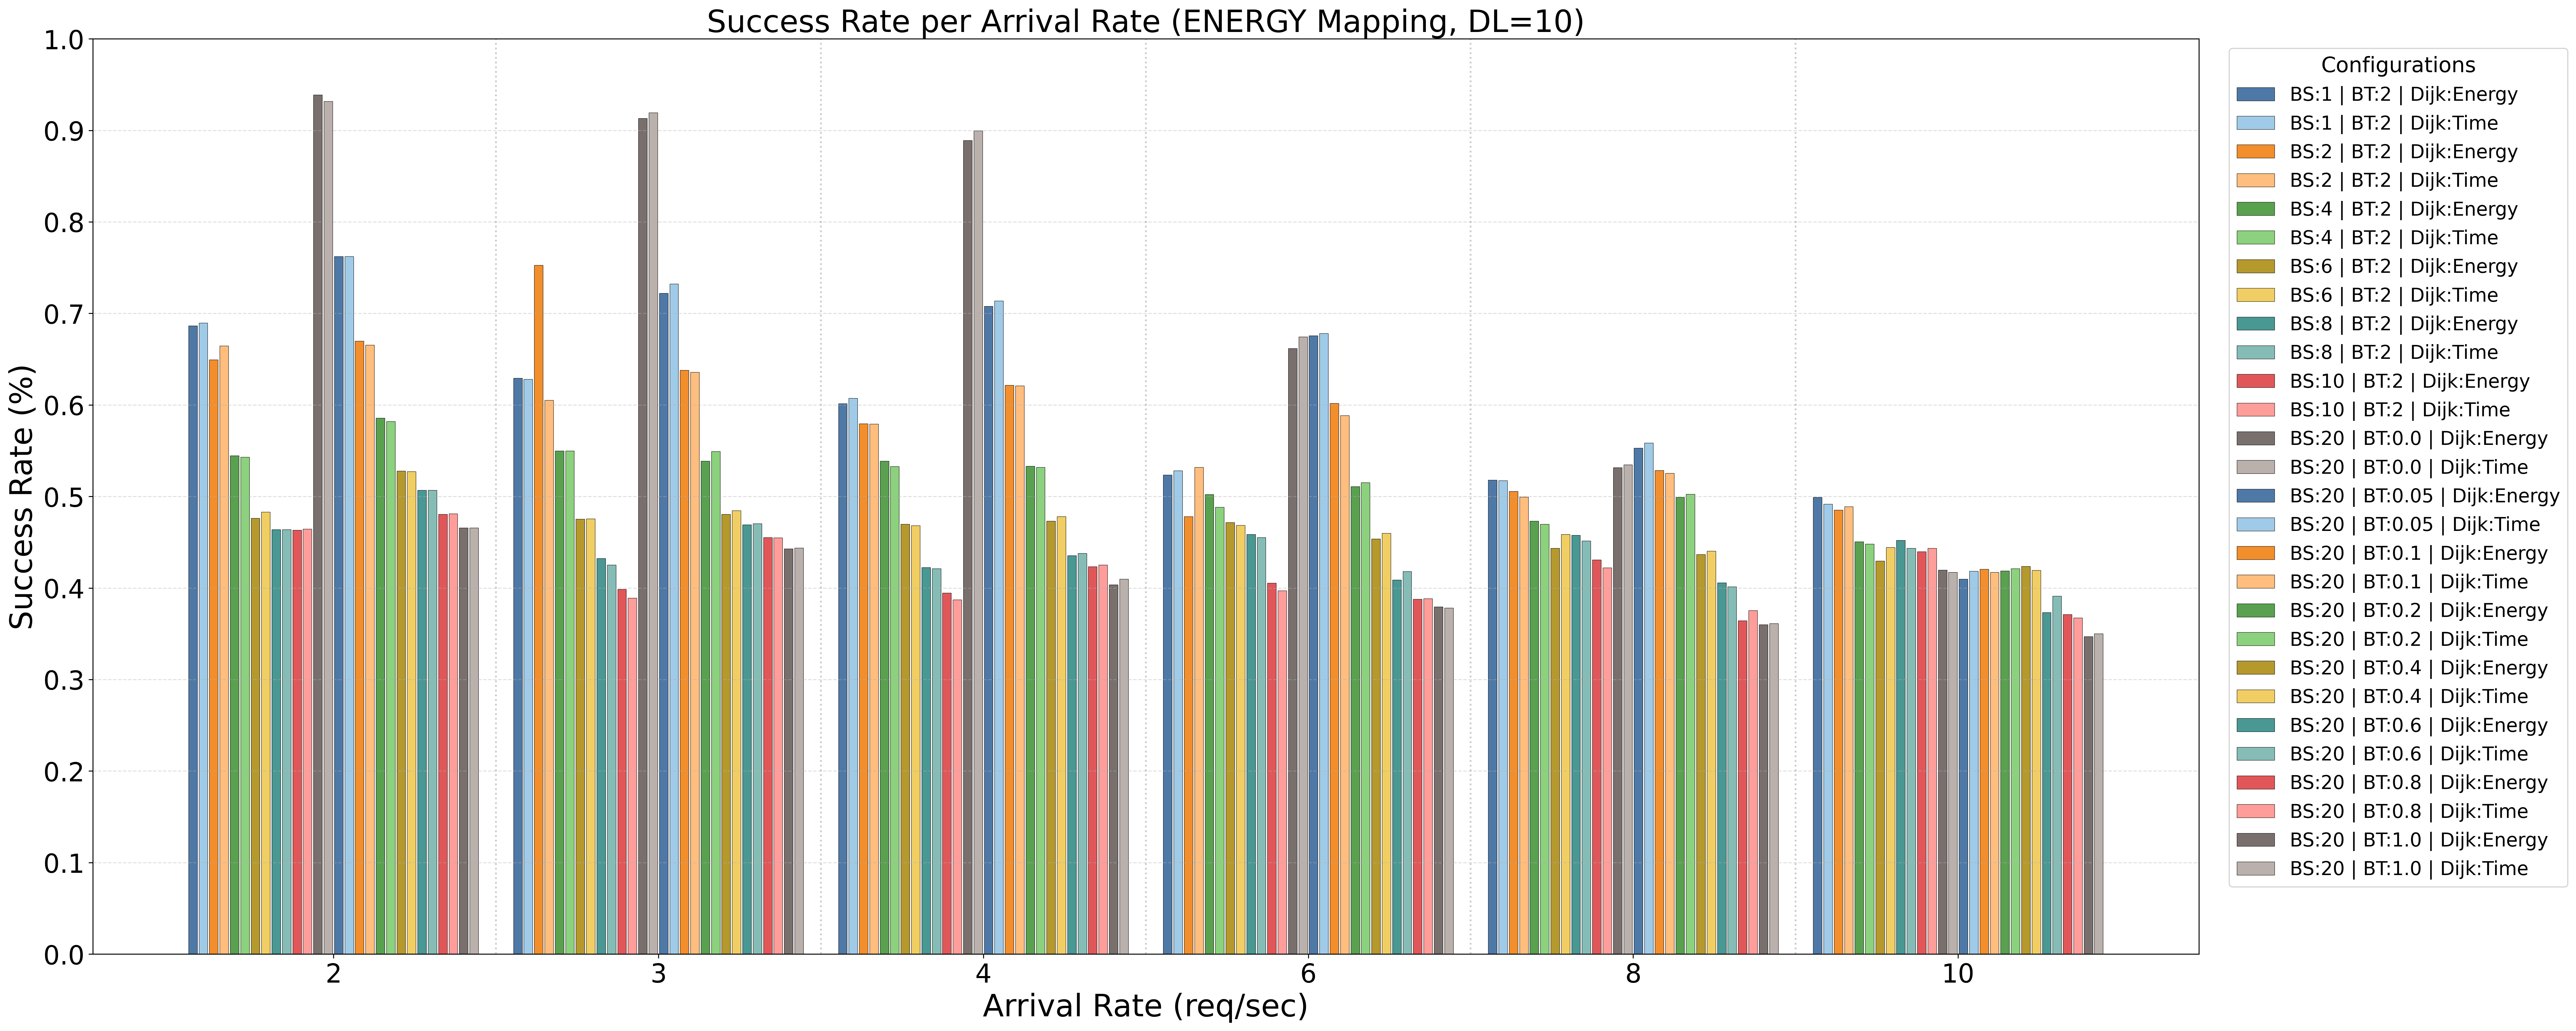
\includegraphics[width=1.3\textwidth]{01_AR_success_rate_energy_dl_10.png}}
        \caption{Scomposizione del Success Rate (DL = 10\%).}
        \label{fig:success_rate_energy_dl_10}
        \end{figure}

        \begin{figure}[H]
        \makebox[\textwidth][c]{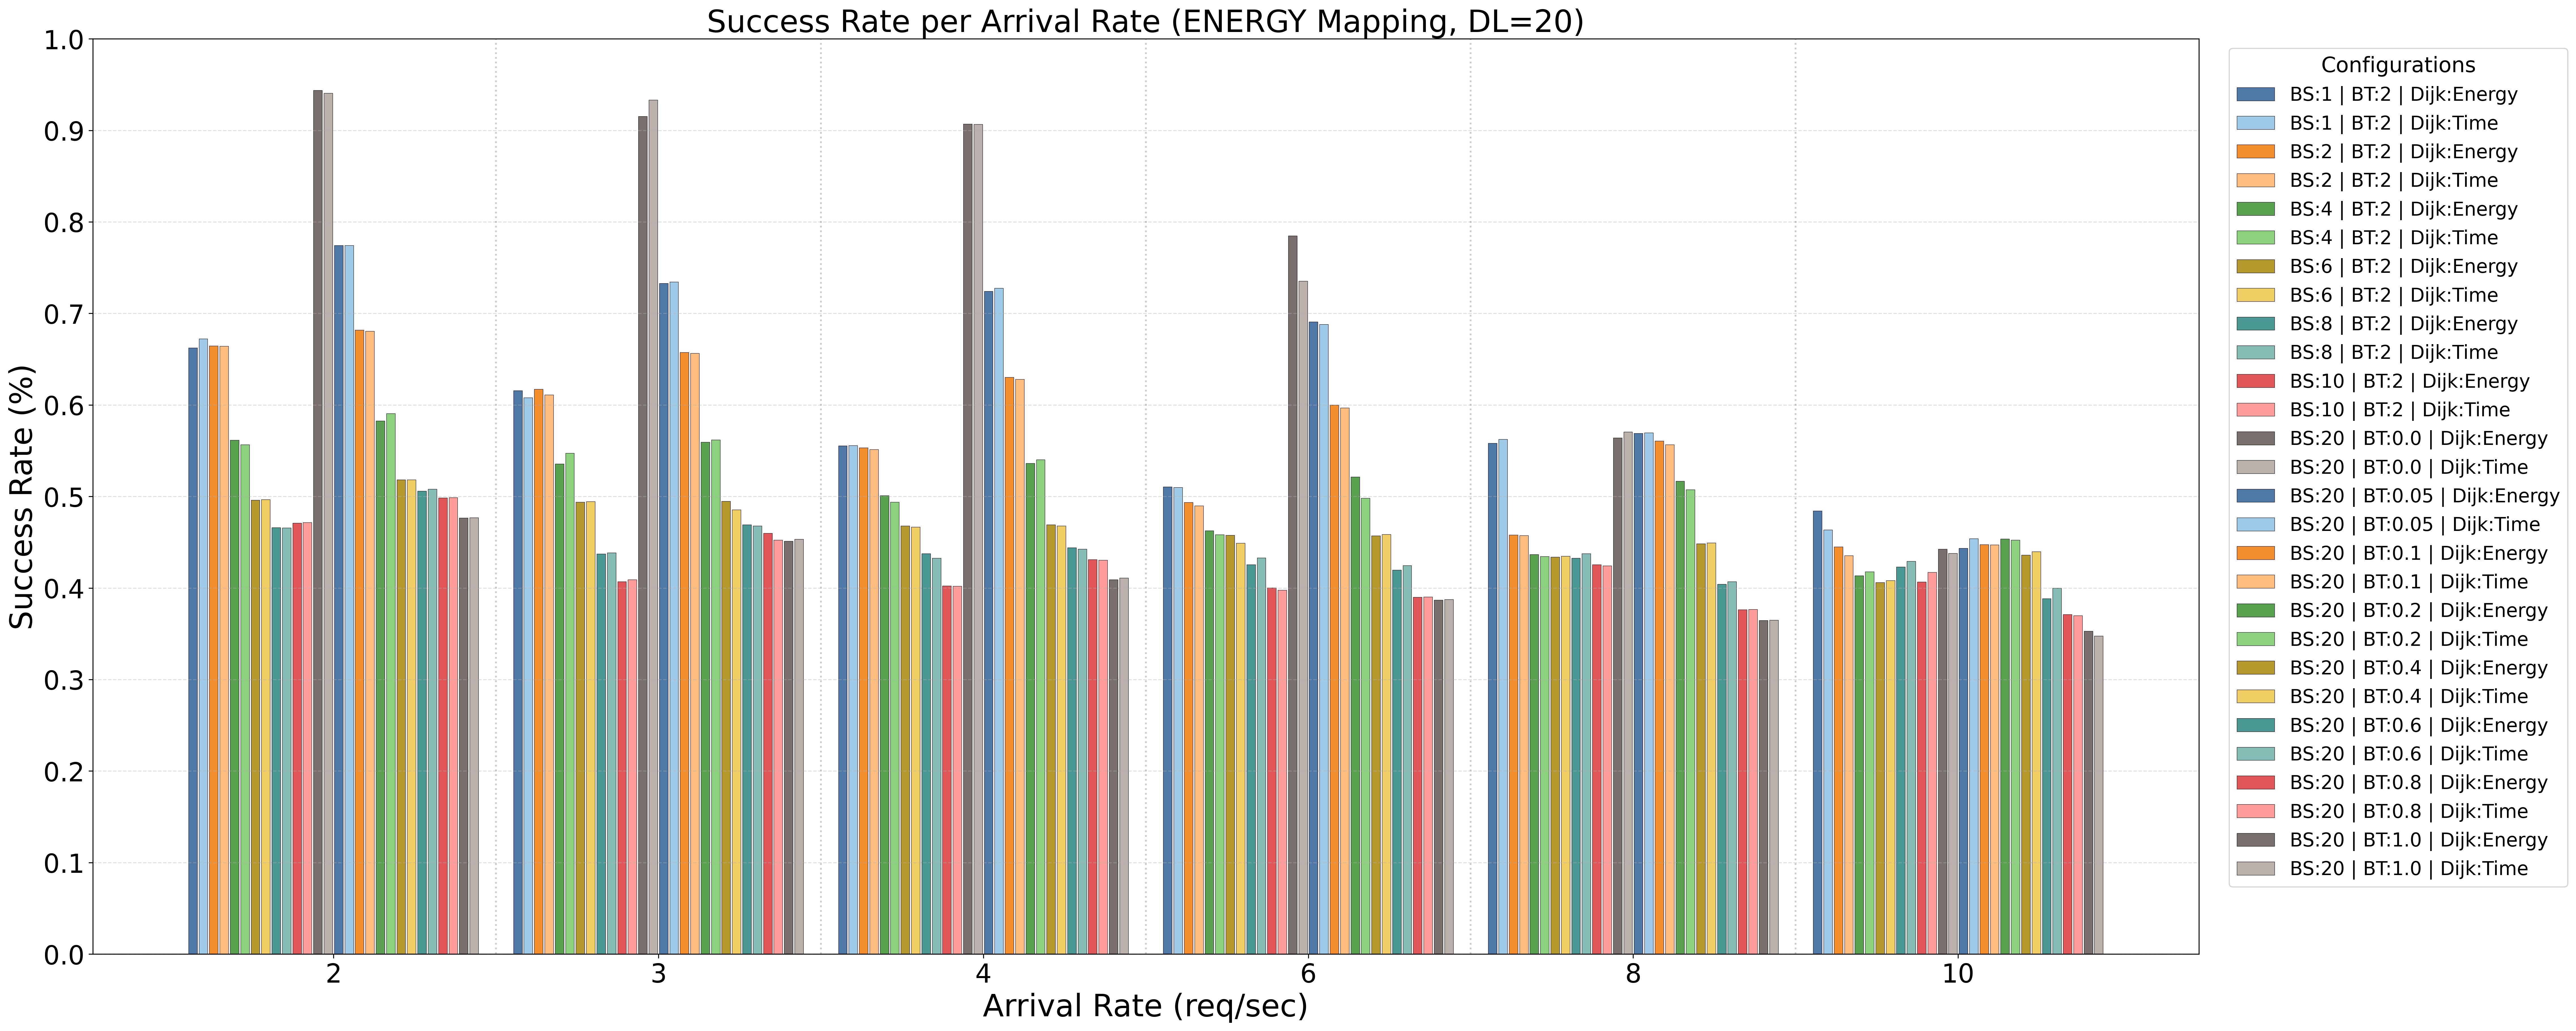
\includegraphics[width=1.3\textwidth]{01_AR_success_rate_energy_dl_20.png}}
        \caption{Scomposizione del Success Rate (DL = 20\%).}
        \label{fig:success_rate_energy_dl_20}
        \end{figure}

        \begin{figure}[H]
        \makebox[\textwidth][c]{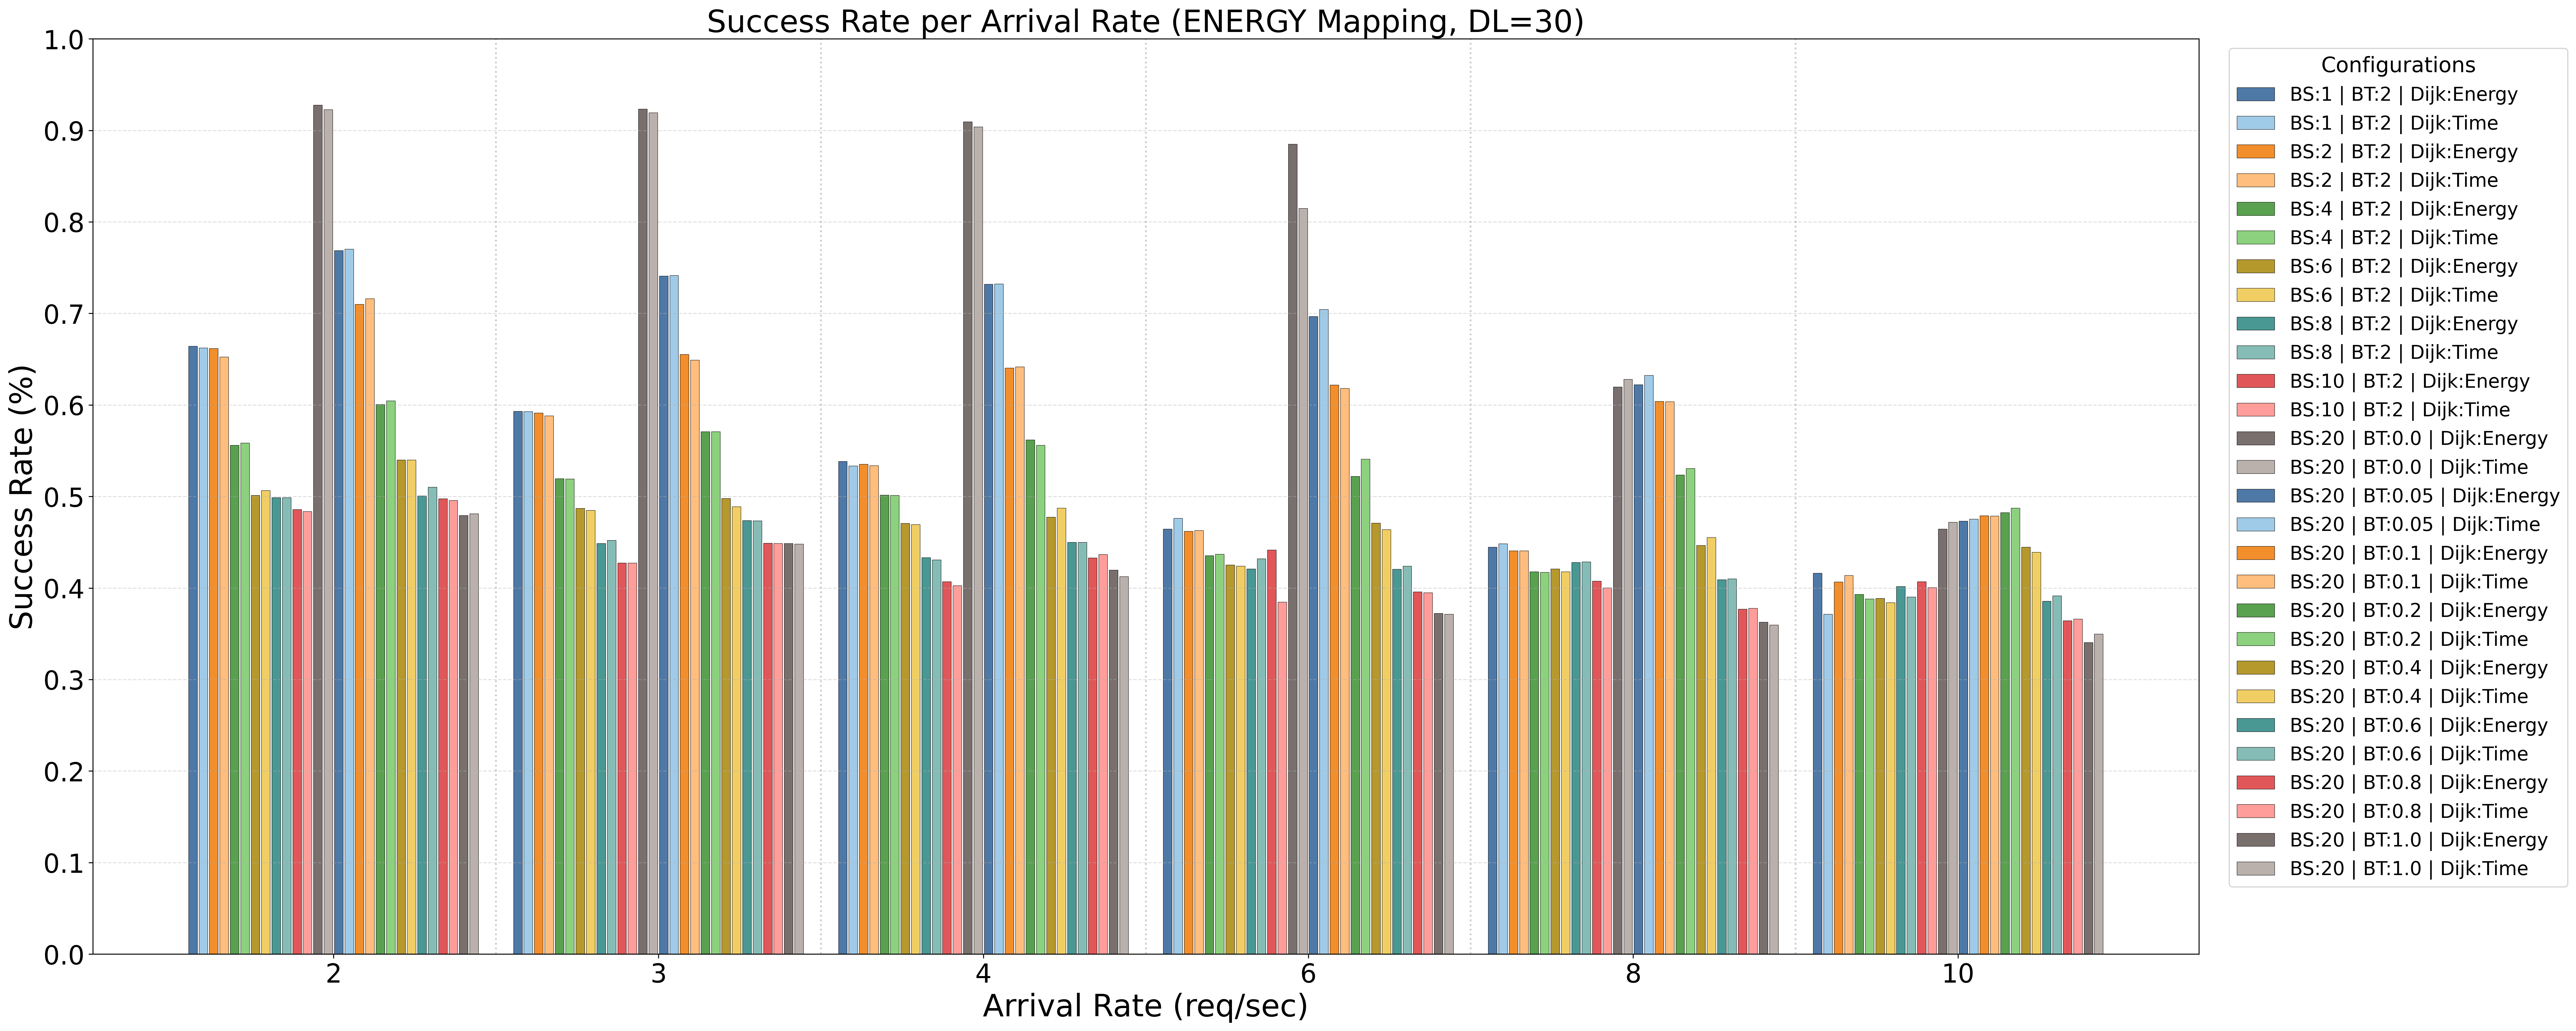
\includegraphics[width=1.3\textwidth]{01_AR_success_rate_energy_dl_30.png}}
        \caption{Scomposizione del Success Rate (DL = 30\%).}
        \label{fig:success_rate_energy_dl_30}
        \end{figure}

        Come si evince dai grafici di Figura \ref{fig:success_rate_energy_dl_10}, \ref{fig:success_rate_energy_dl_20} e \ref{fig:success_rate_energy_dl_30}, un incremento del parametro di rilassamento della deadline non produce, in generale, un aumento significativo del tasso di successo delle richieste. Tuttavia, in specifiche configurazioni si registra un lieve miglioramento prestazionale. Spicca, in particolare, l'impostazione con BS = 20 e BT = 0.0, che mostra una crescita del tasso di successo di circa il 10\% passando da DL = 10\% a DL = 30\%.
        Risulta invece anomalo il divario prestazionale della configurazione con BS = 1 e BT = 2.0, la quale presenta un tasso di successo nettamente inferiore rispetto al caso BS = 20 e BT = 0.0. L'ipotesi più plausibile per spiegare tale comportamento è da ricercarsi nelle dinamiche interne di gestione degli eventi da parte dell'ambiente SimPy.

    \subsection{Rejection Reasons}

        \begin{figure}[H]
        \makebox[\textwidth][c]{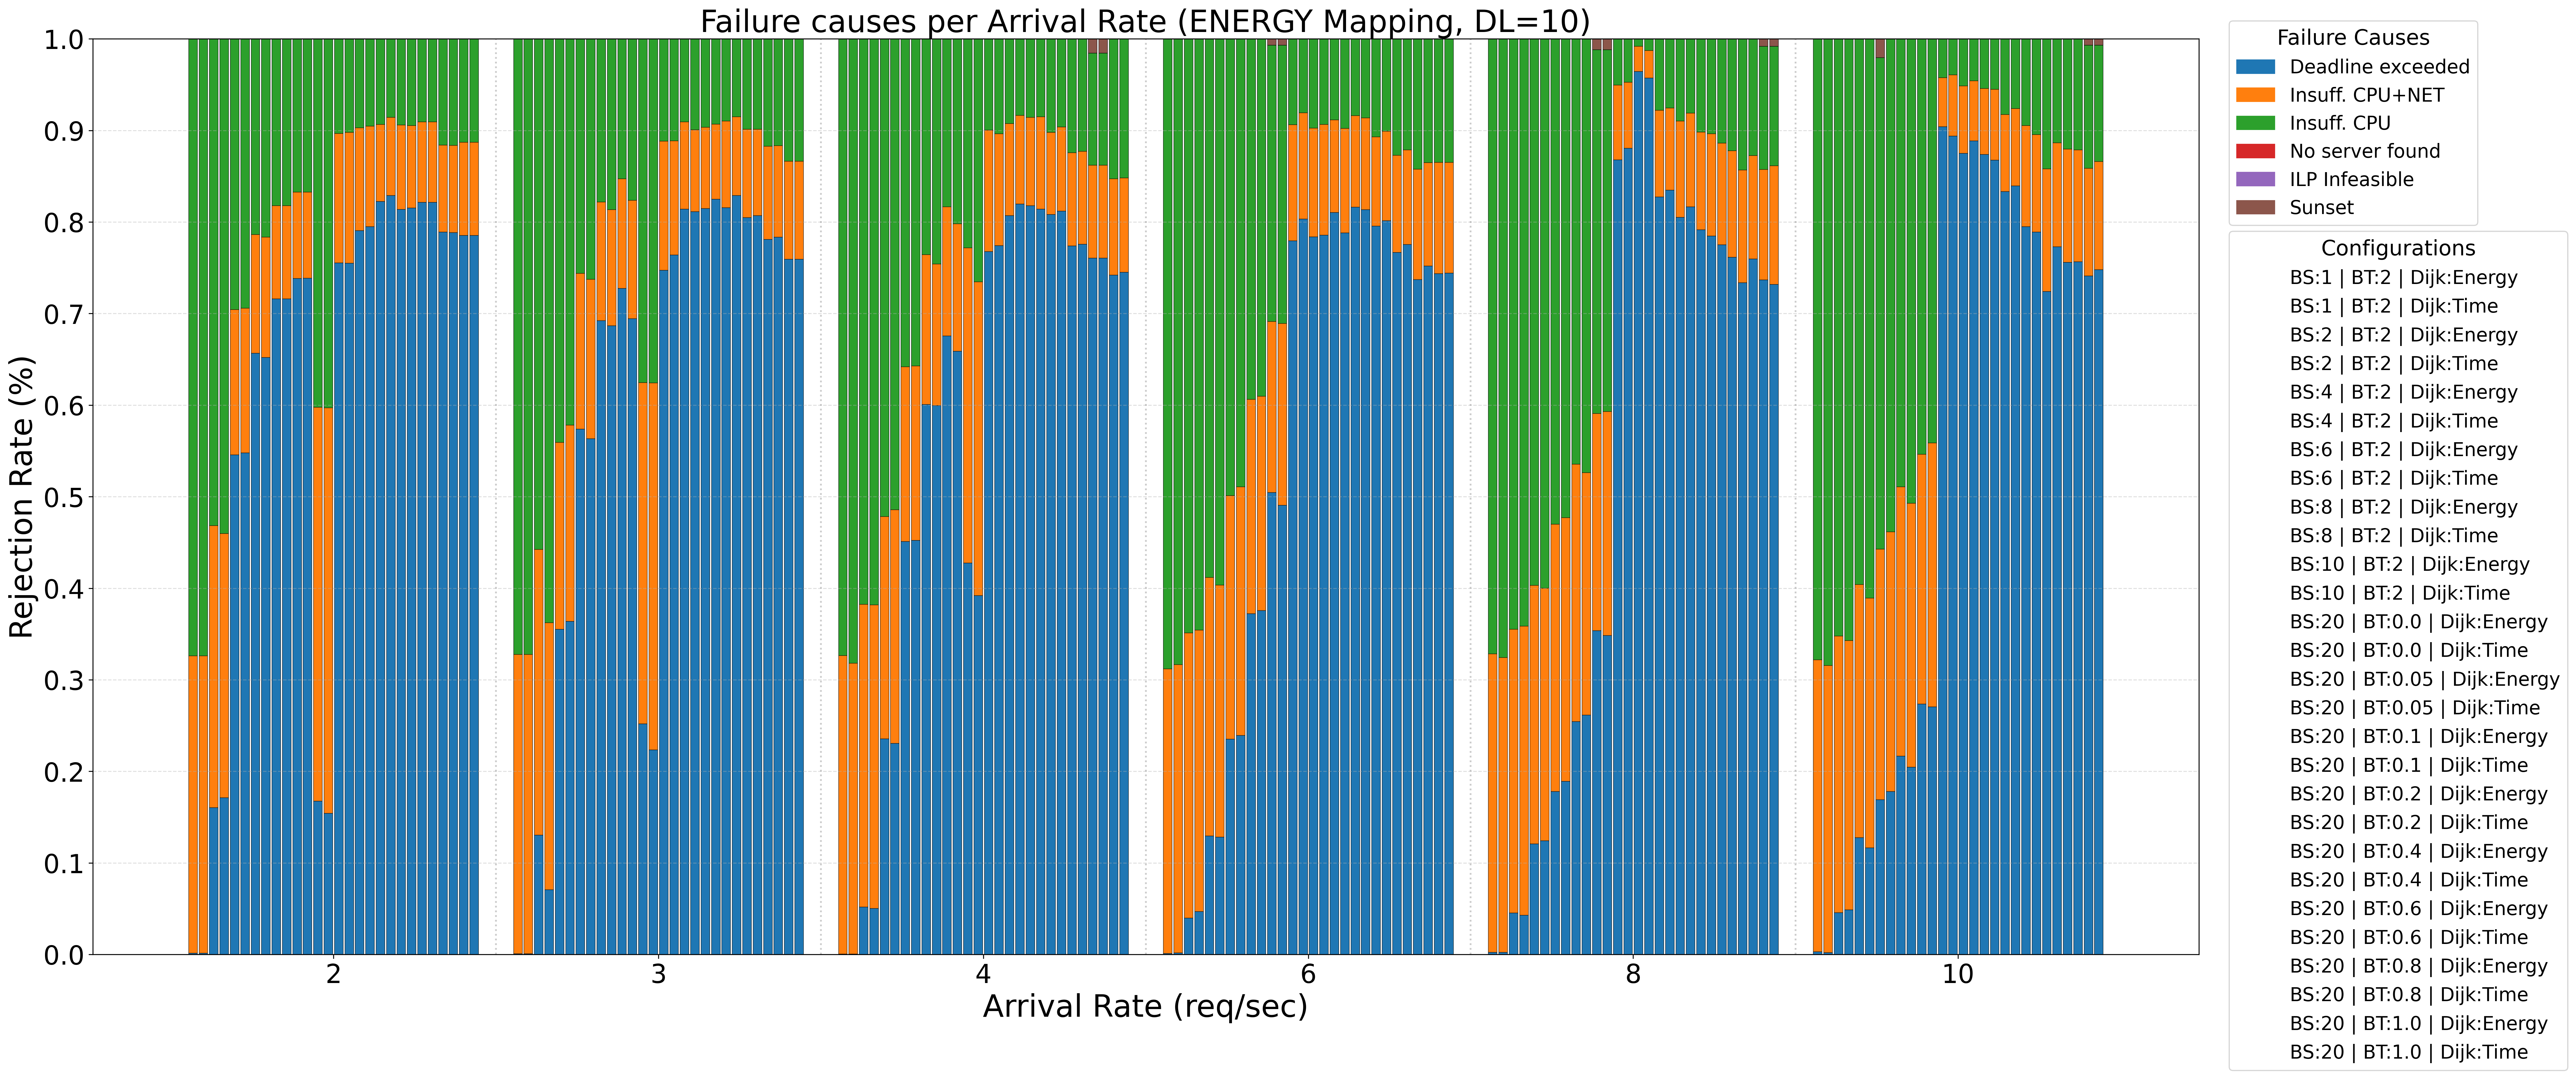
\includegraphics[width=1.3\textwidth]{02_AR_rejection_energy_dl_10.png}}
        \caption{Scomposizione del Rejection Reasons (DL = 10\%).}
        \label{fig:rejection_rate_energy_dl_10}
        \end{figure}

        \begin{figure}[H]
        \makebox[\textwidth][c]{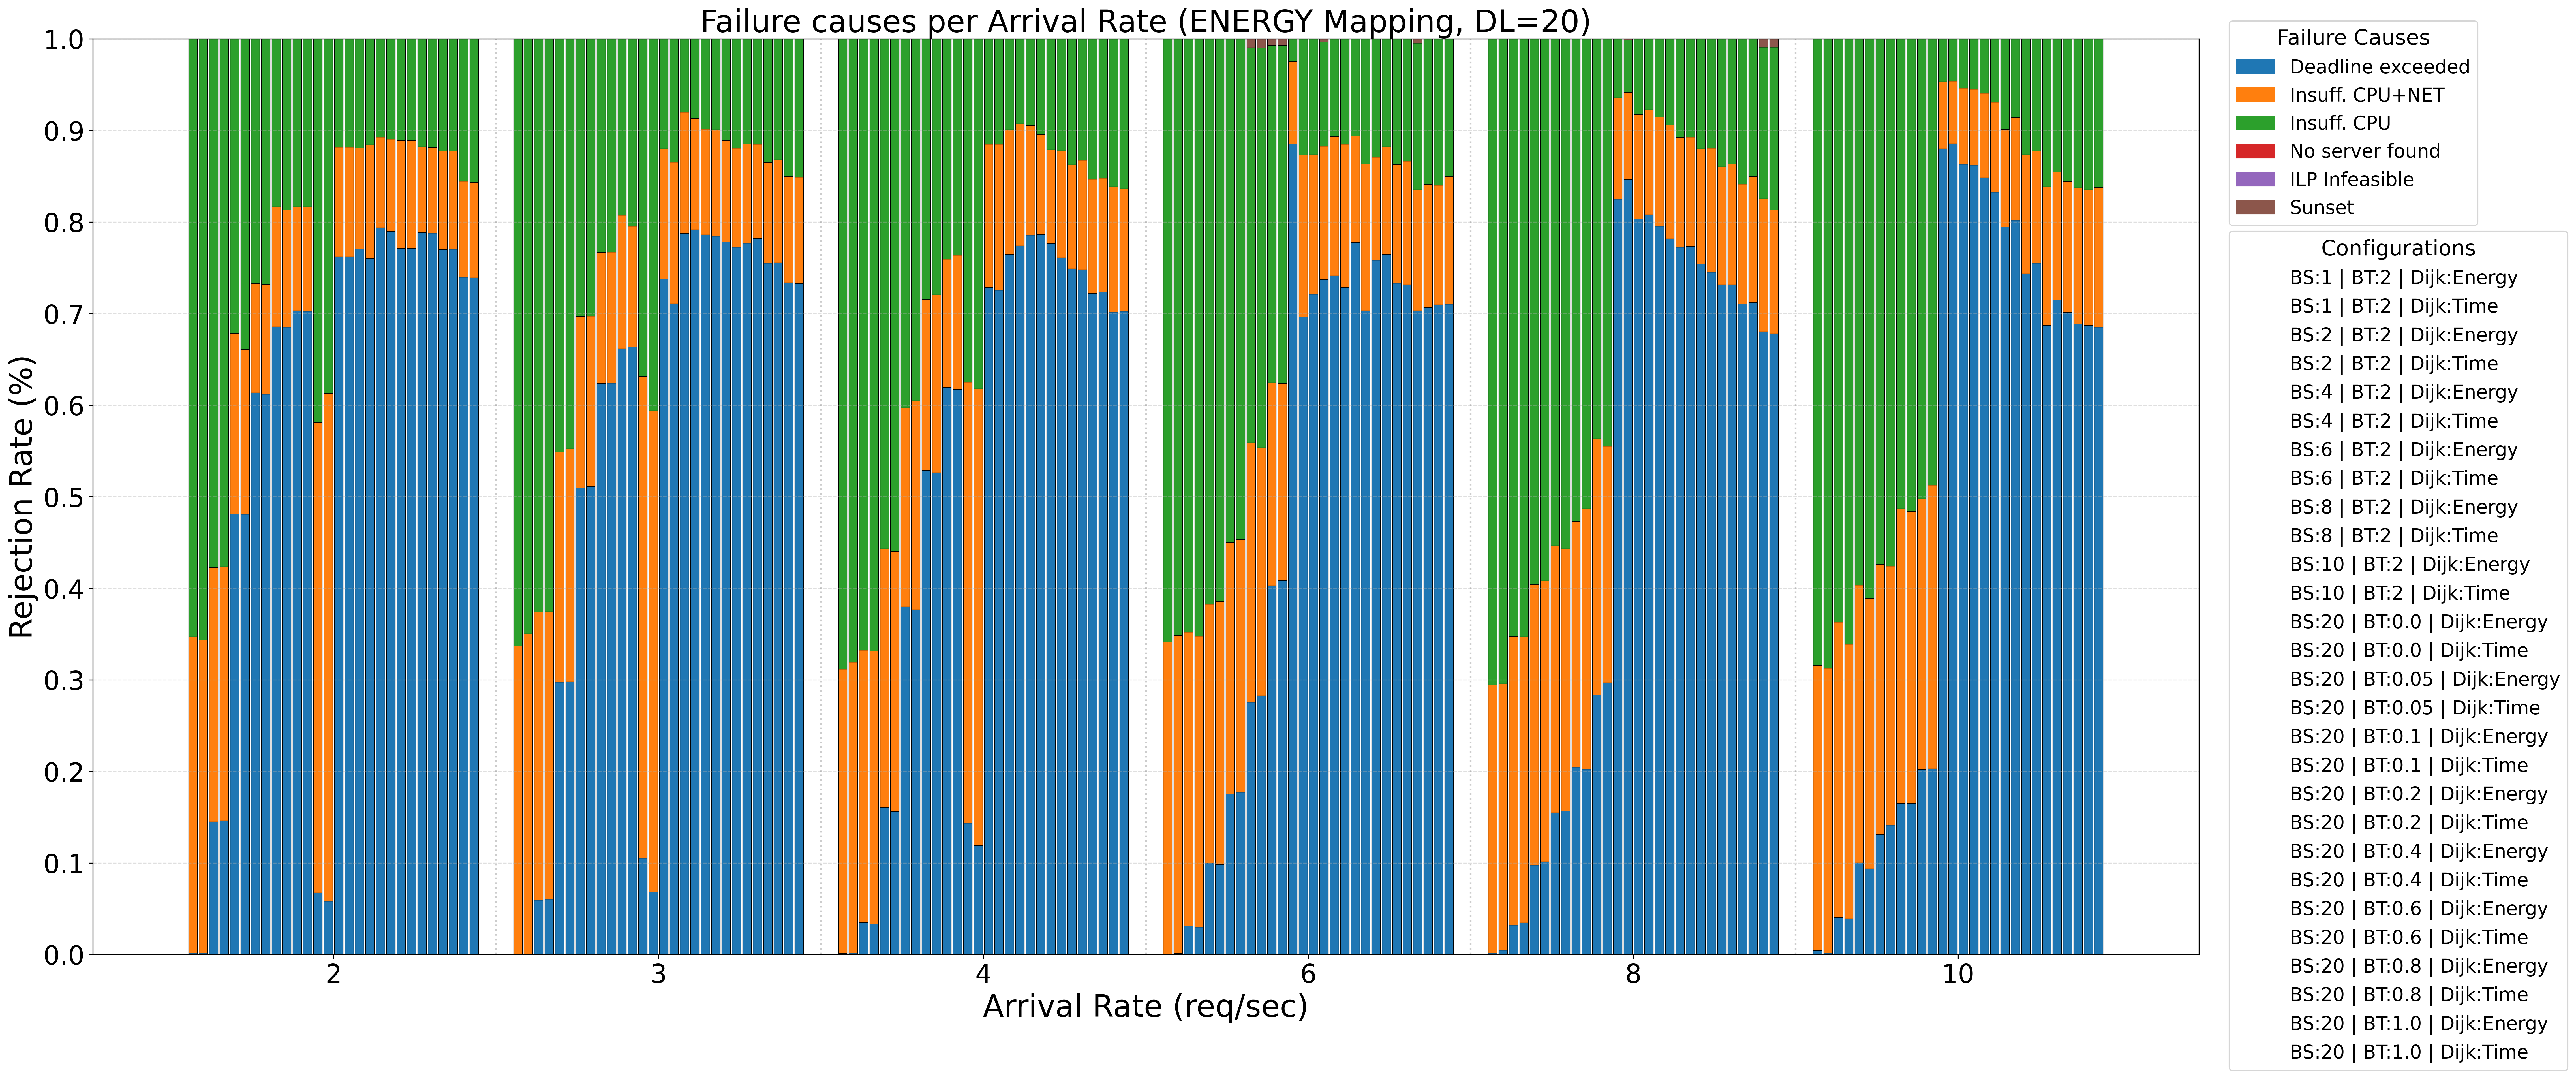
\includegraphics[width=1.3\textwidth]{02_AR_rejection_energy_dl_20.png}}
        \caption{Scomposizione del Rejection Reasons (DL = 20\%).}
        \label{fig:rejection_rate_energy_dl_20}
        \end{figure}

        \begin{figure}[H]
        \makebox[\textwidth][c]{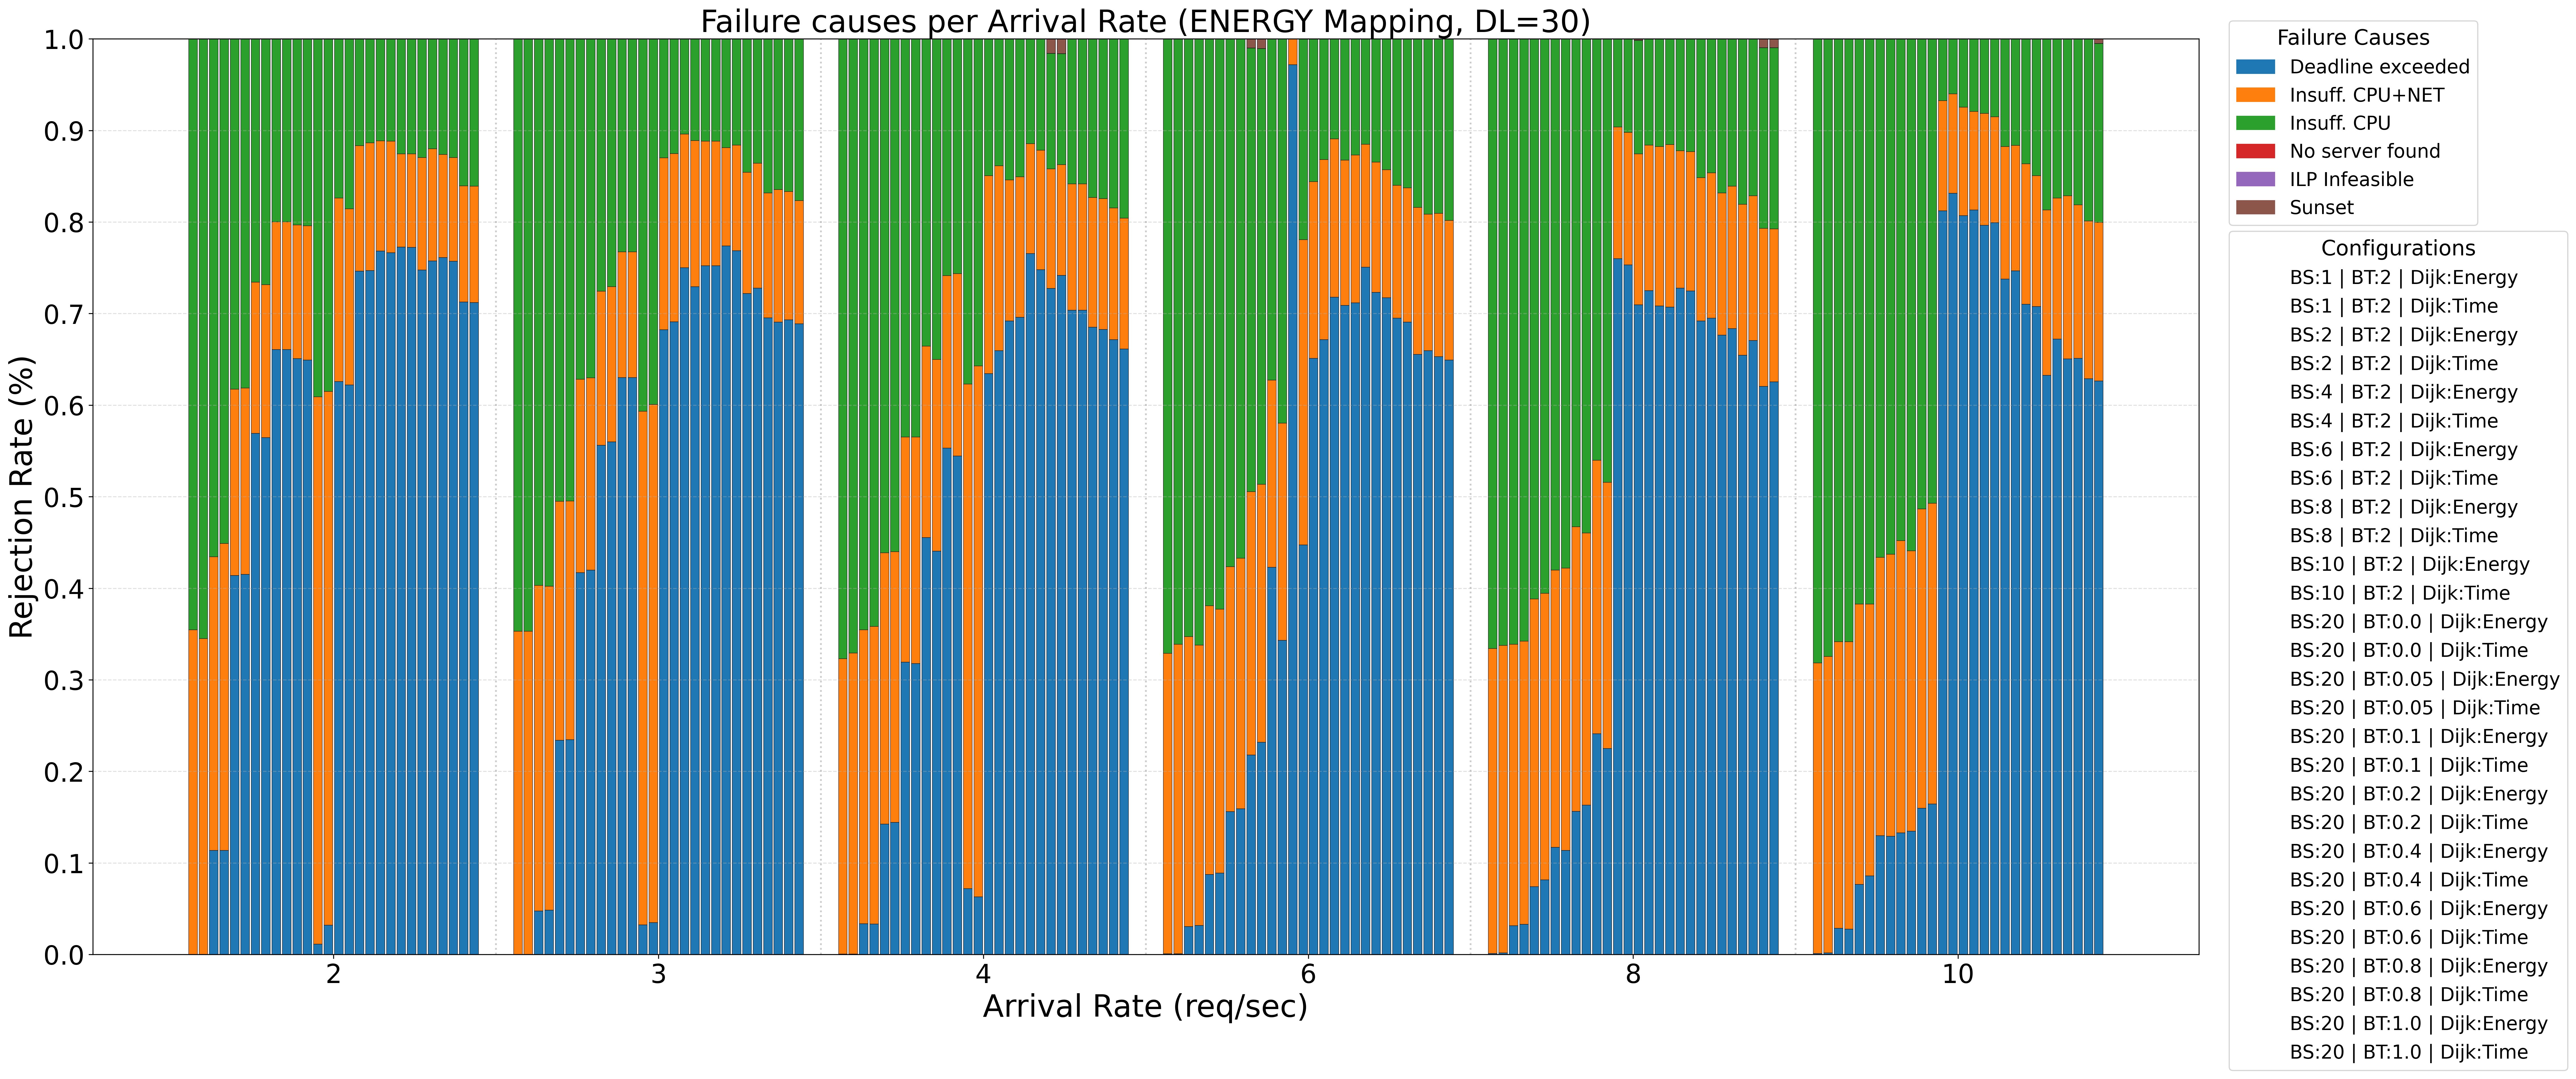
\includegraphics[width=1.3\textwidth]{02_AR_rejection_energy_dl_30.png}}
        \caption{Scomposizione del Rejection Reasons (DL = 30\%).}
        \label{fig:rejection_rate_energy_dl_30}
        \end{figure}

        L'analisi delle Figure \ref{fig:rejection_rate_energy_dl_10}, \ref{fig:rejection_rate_energy_dl_20} e \ref{fig:rejection_rate_energy_dl_30} mostra come l'incremento del parametro di rilassamento della deadline (DL) alteri significativamente la distribuzione delle cause di reiezione. Nello specifico, passando da un DL del 10\% al 30\%, diminuiscono i fallimenti per superamento del limite temporale (\textit{Deadline exceeded}), grazie al maggior margine a disposizione per l'allocazione.

        Tuttavia, tale riduzione è interamente compensata da un proporzionale aumento delle reiezioni per esaurimento capacitivo (\textit{Insuff. CPU} e \textit{Insuff. CPU/NET}): trattenendo le richieste nel sistema per un tempo maggiore, si accelera infatti la saturazione delle risorse fisiche. Infine, all'aumentare del carico (\textit{Arrival Rate}), la carenza infrastrutturale si consolida strutturalmente come il principale collo di bottiglia del sistema, scavalcando i limiti imposti dalla latenza.

    \subsection{Response Time}


        \begin{figure}[H]
        \makebox[\textwidth][c]{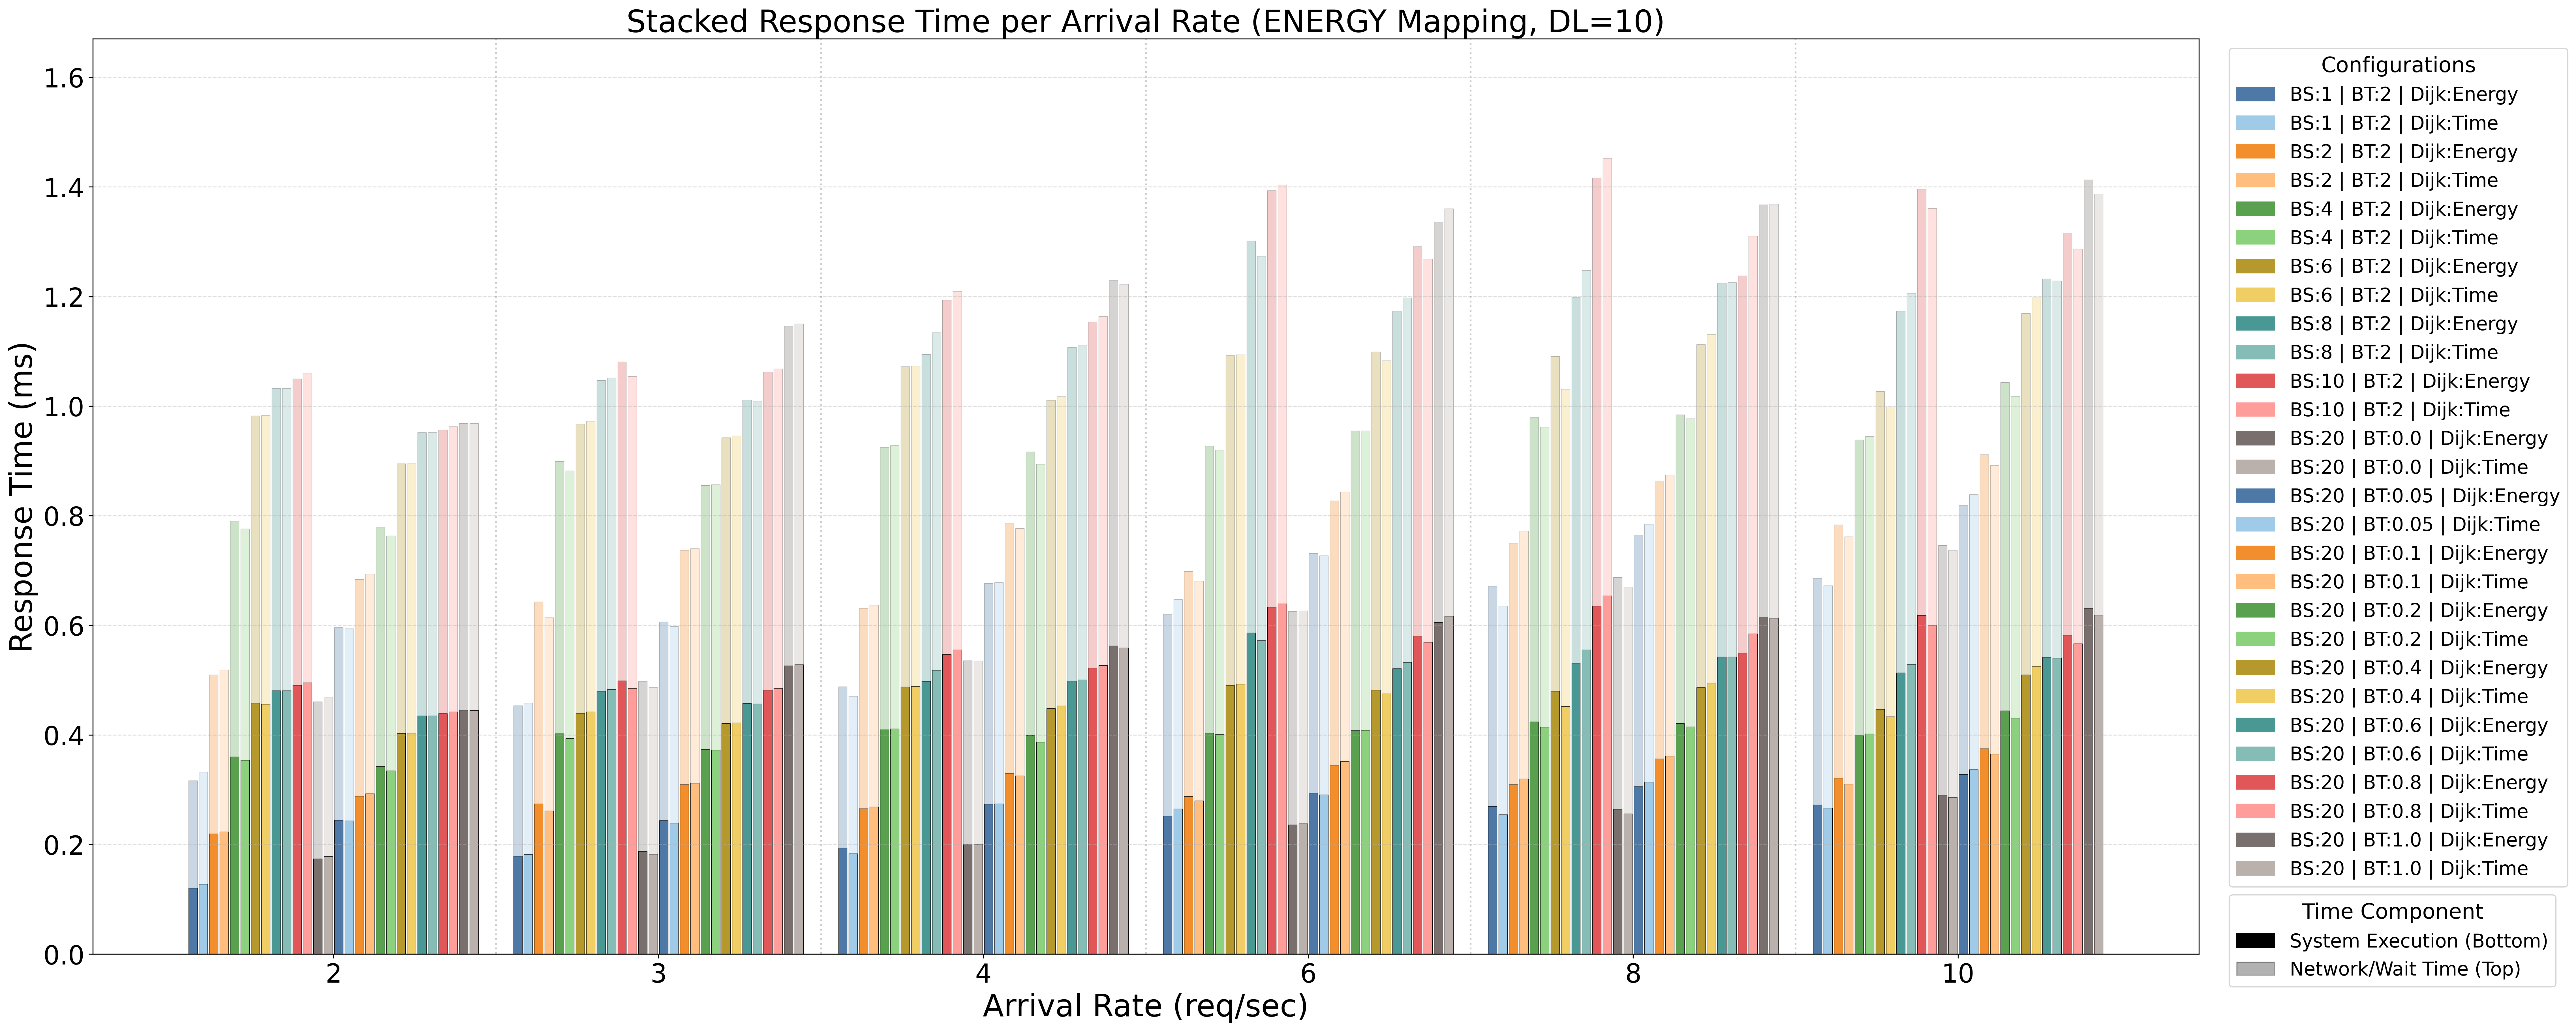
\includegraphics[width=1.3\textwidth]{03_AR_response_energy_dl_10.png}}
        \caption{Scomposizione del Response Time (DL = 10\%).}
        \label{fig:response_time_energy_dl_10}
        \end{figure}

        \begin{figure}[H]
        \makebox[\textwidth][c]{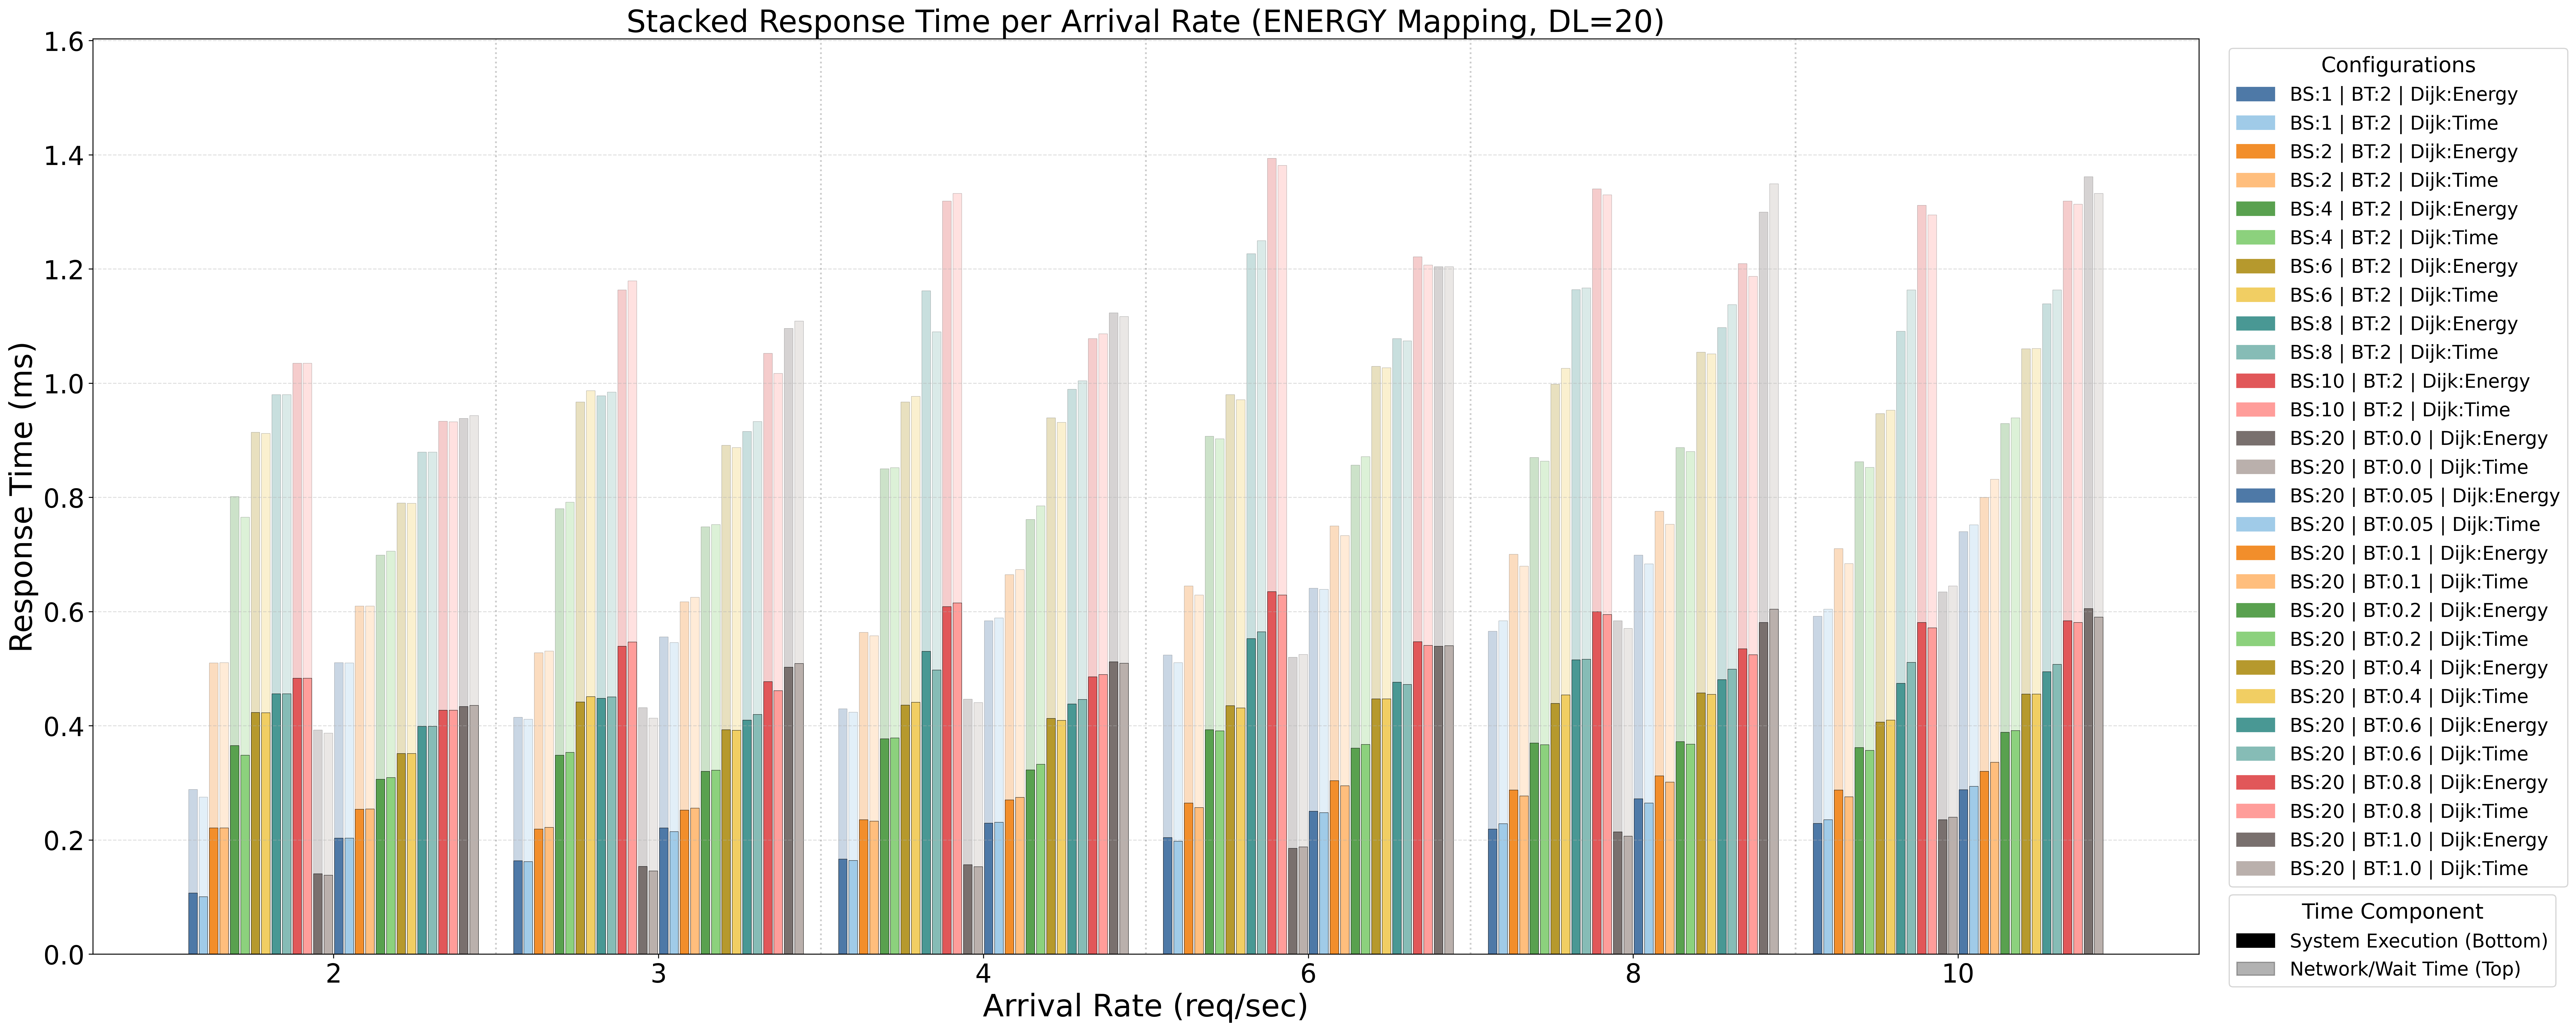
\includegraphics[width=1.3\textwidth]{03_AR_response_energy_dl_20.png}}
        \caption{Scomposizione del Response Time (DL = 20\%).}
        \label{fig:response_time_energy_dl_20}
        \end{figure}

        \begin{figure}[H]
        \makebox[\textwidth][c]{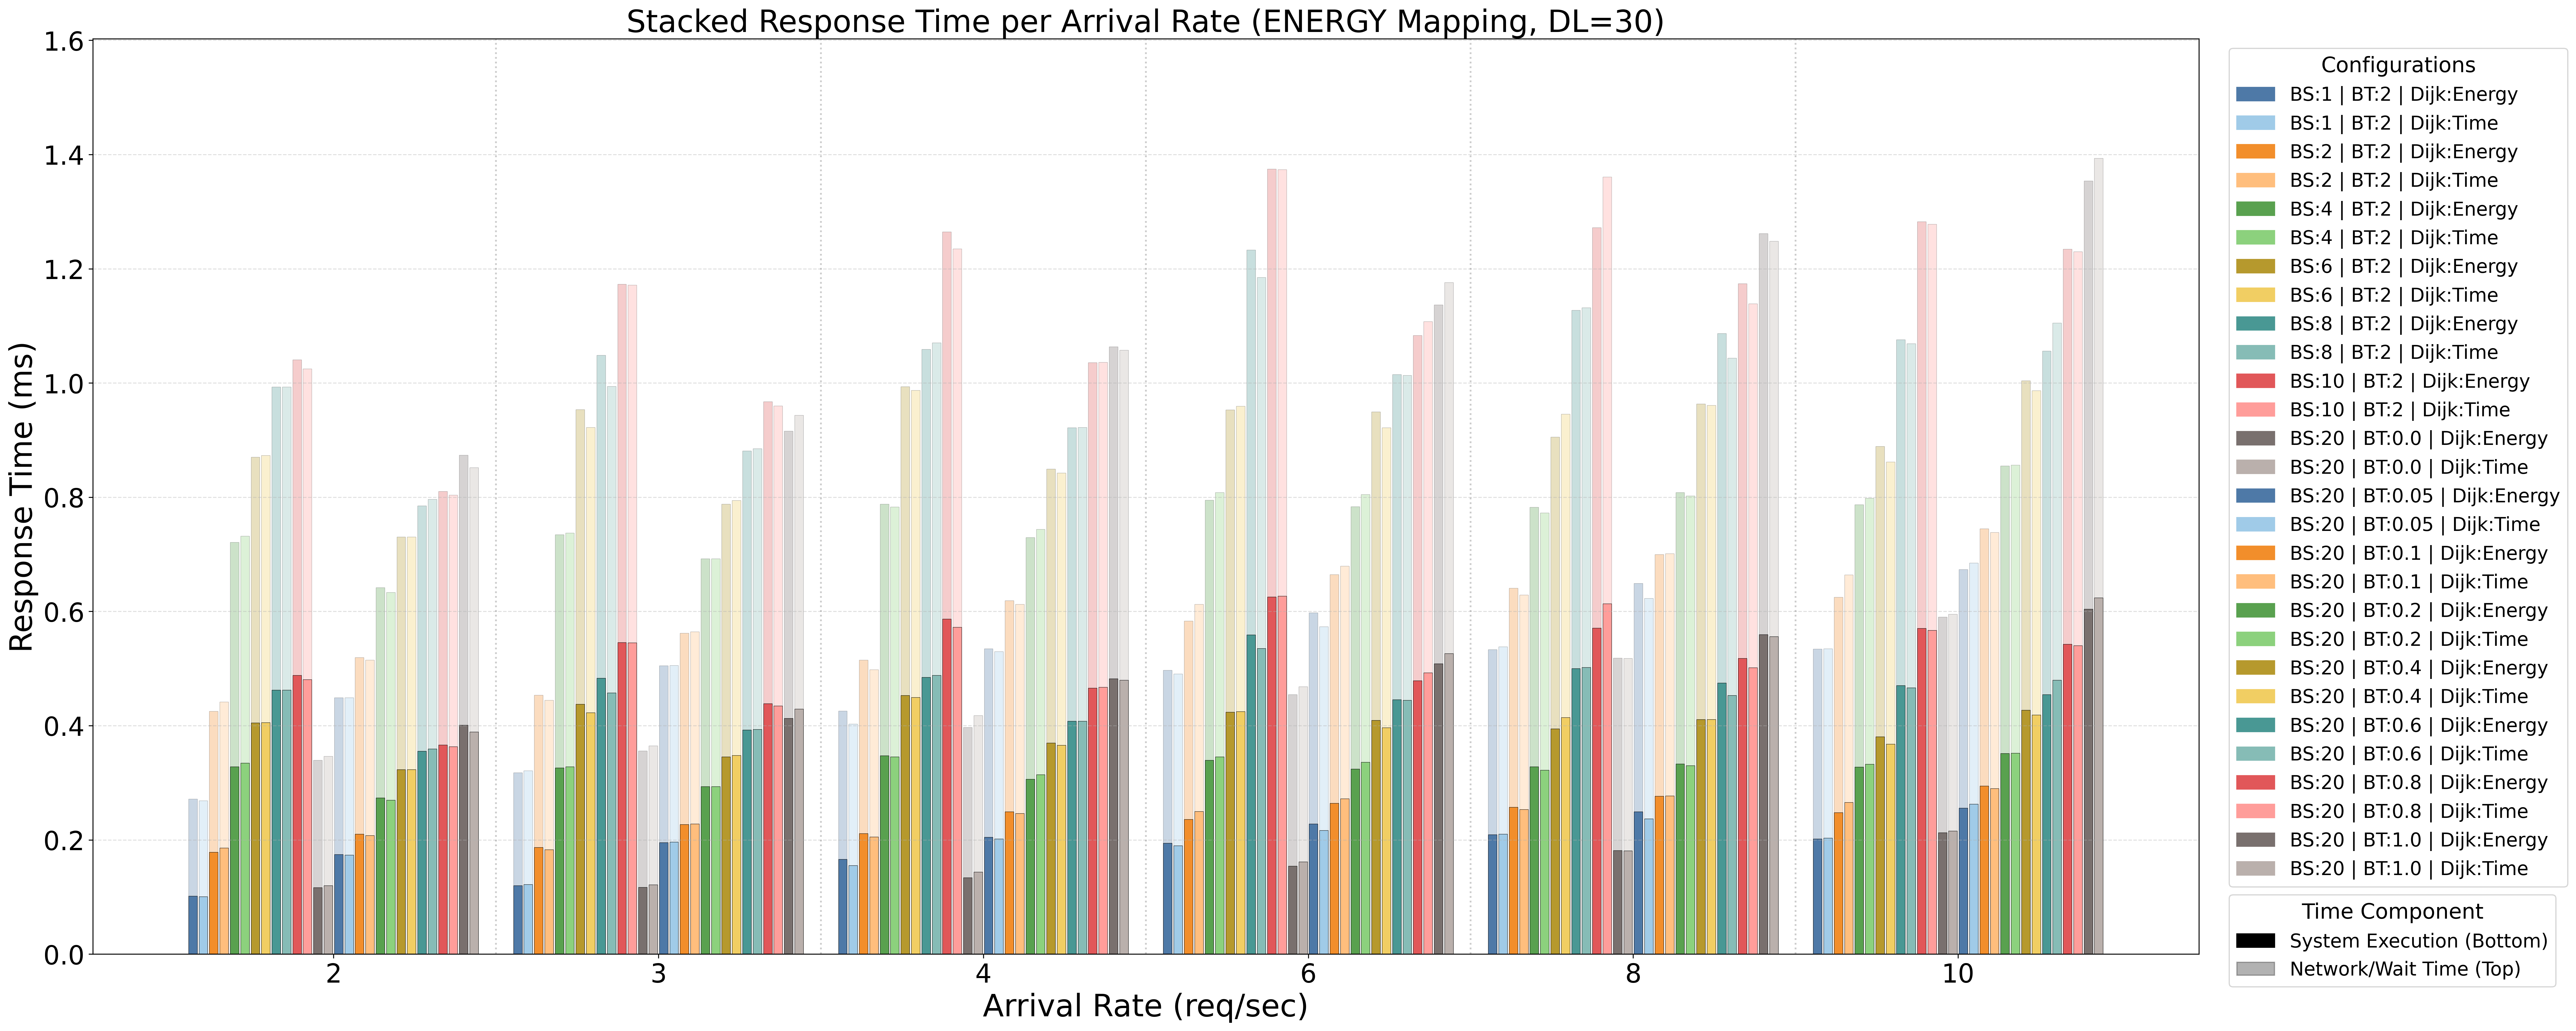
\includegraphics[width=1.3\textwidth]{03_AR_response_energy_dl_30.png}}
        \caption{Scomposizione del Response Time (DL = 30\%).}
        \label{fig:response_time_energy_dl_30}
        \end{figure}

        Come si evince dall'analisi delle Figure \ref{fig:response_time_energy_dl_10}, \ref{fig:response_time_energy_dl_20} e \ref{fig:response_time_energy_dl_30}, relative all'andamento dei tempi di risposta, un incremento del carico di richieste (\textit{Arrival Rate}) produce un prevedibile innalzamento delle latenze complessive. La scomposizione del grafico a barre impilate evidenzia chiaramente come il tempo totale sia ampiamente dominato dalla componente di rete (\textit{Network/Wait Time}, porzione superiore sbiadita), mentre i tempi di elaborazione vera e propria del sistema (\textit{System Execution}, porzione inferiore solida) si mantengano marginali e pressoché costanti.

        Infine, la variazione del rilassamento della deadline (DL dal 10\% al 30\%) non altera in modo sostanziale queste dinamiche.


\section{Configurazione Time}

    La variazione dei risultati sperimentali tra le 2 configurazioni di \textit{Objective Mapping} (Energy vs Time) è stata sorprendentemente minima. In generale, la configurazione \textit{Mapping Time} ha mostrato un leggero miglioramento del tasso di successo delle richieste, con una riduzione del tempo medio di risposta. Tuttavia, le differenze non sono state così marcate da giustificare un cambiamento radicale nella strategia di mappatura.

    \subsection{Success Rate}

        \begin{figure}[H]
        \makebox[\textwidth][c]{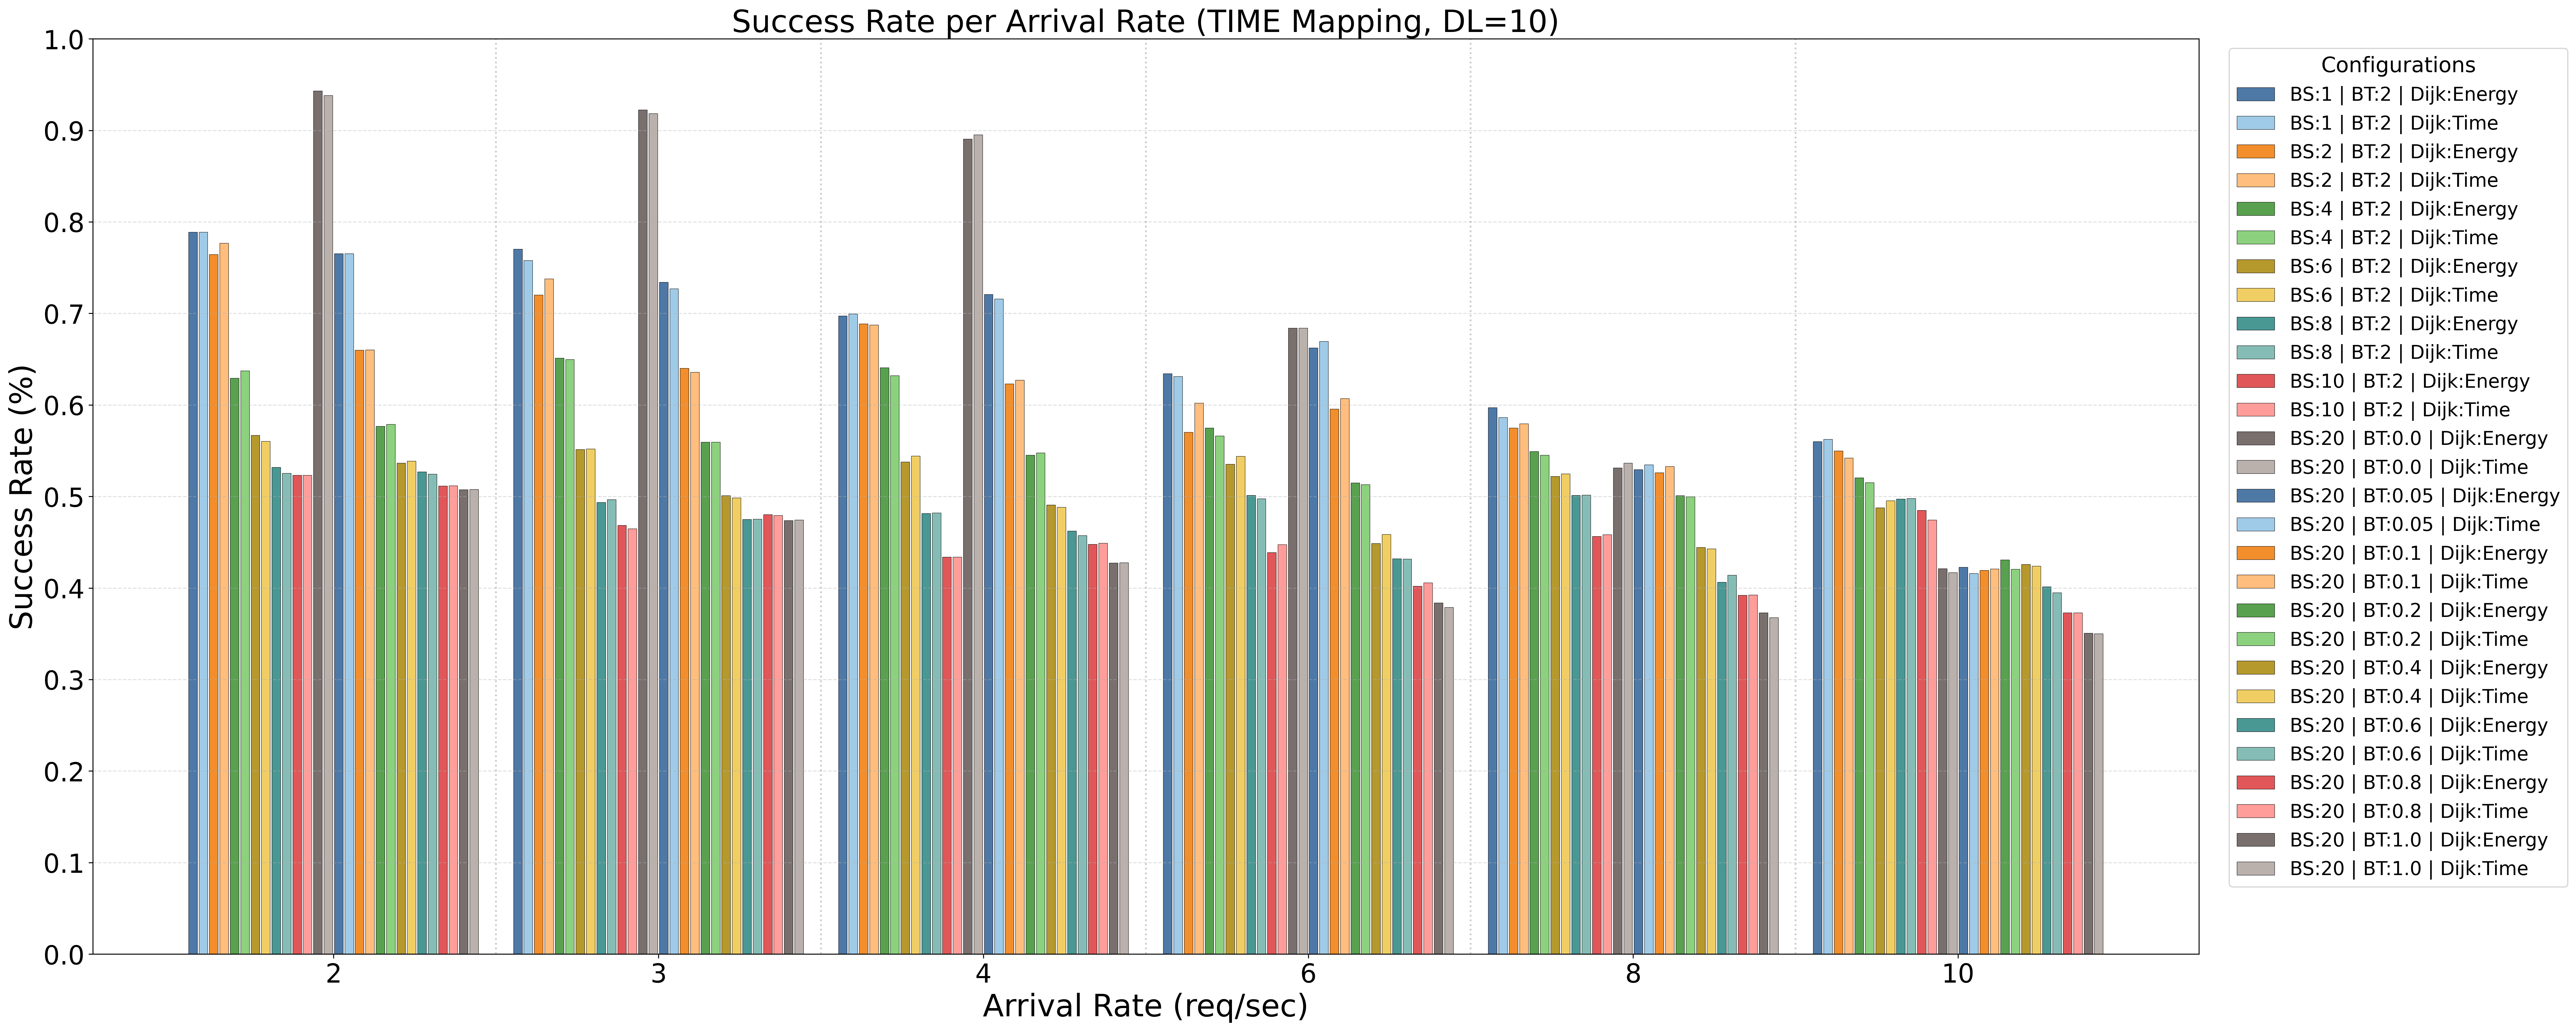
\includegraphics[width=1.3\textwidth]{01_AR_success_rate_time_dl_10.png}}
        \caption{Scomposizione del Success Rate (DL = 10\%).}
        \label{fig:success_rate_time_dl_10}
        \end{figure}

        \begin{figure}[H]
        \makebox[\textwidth][c]{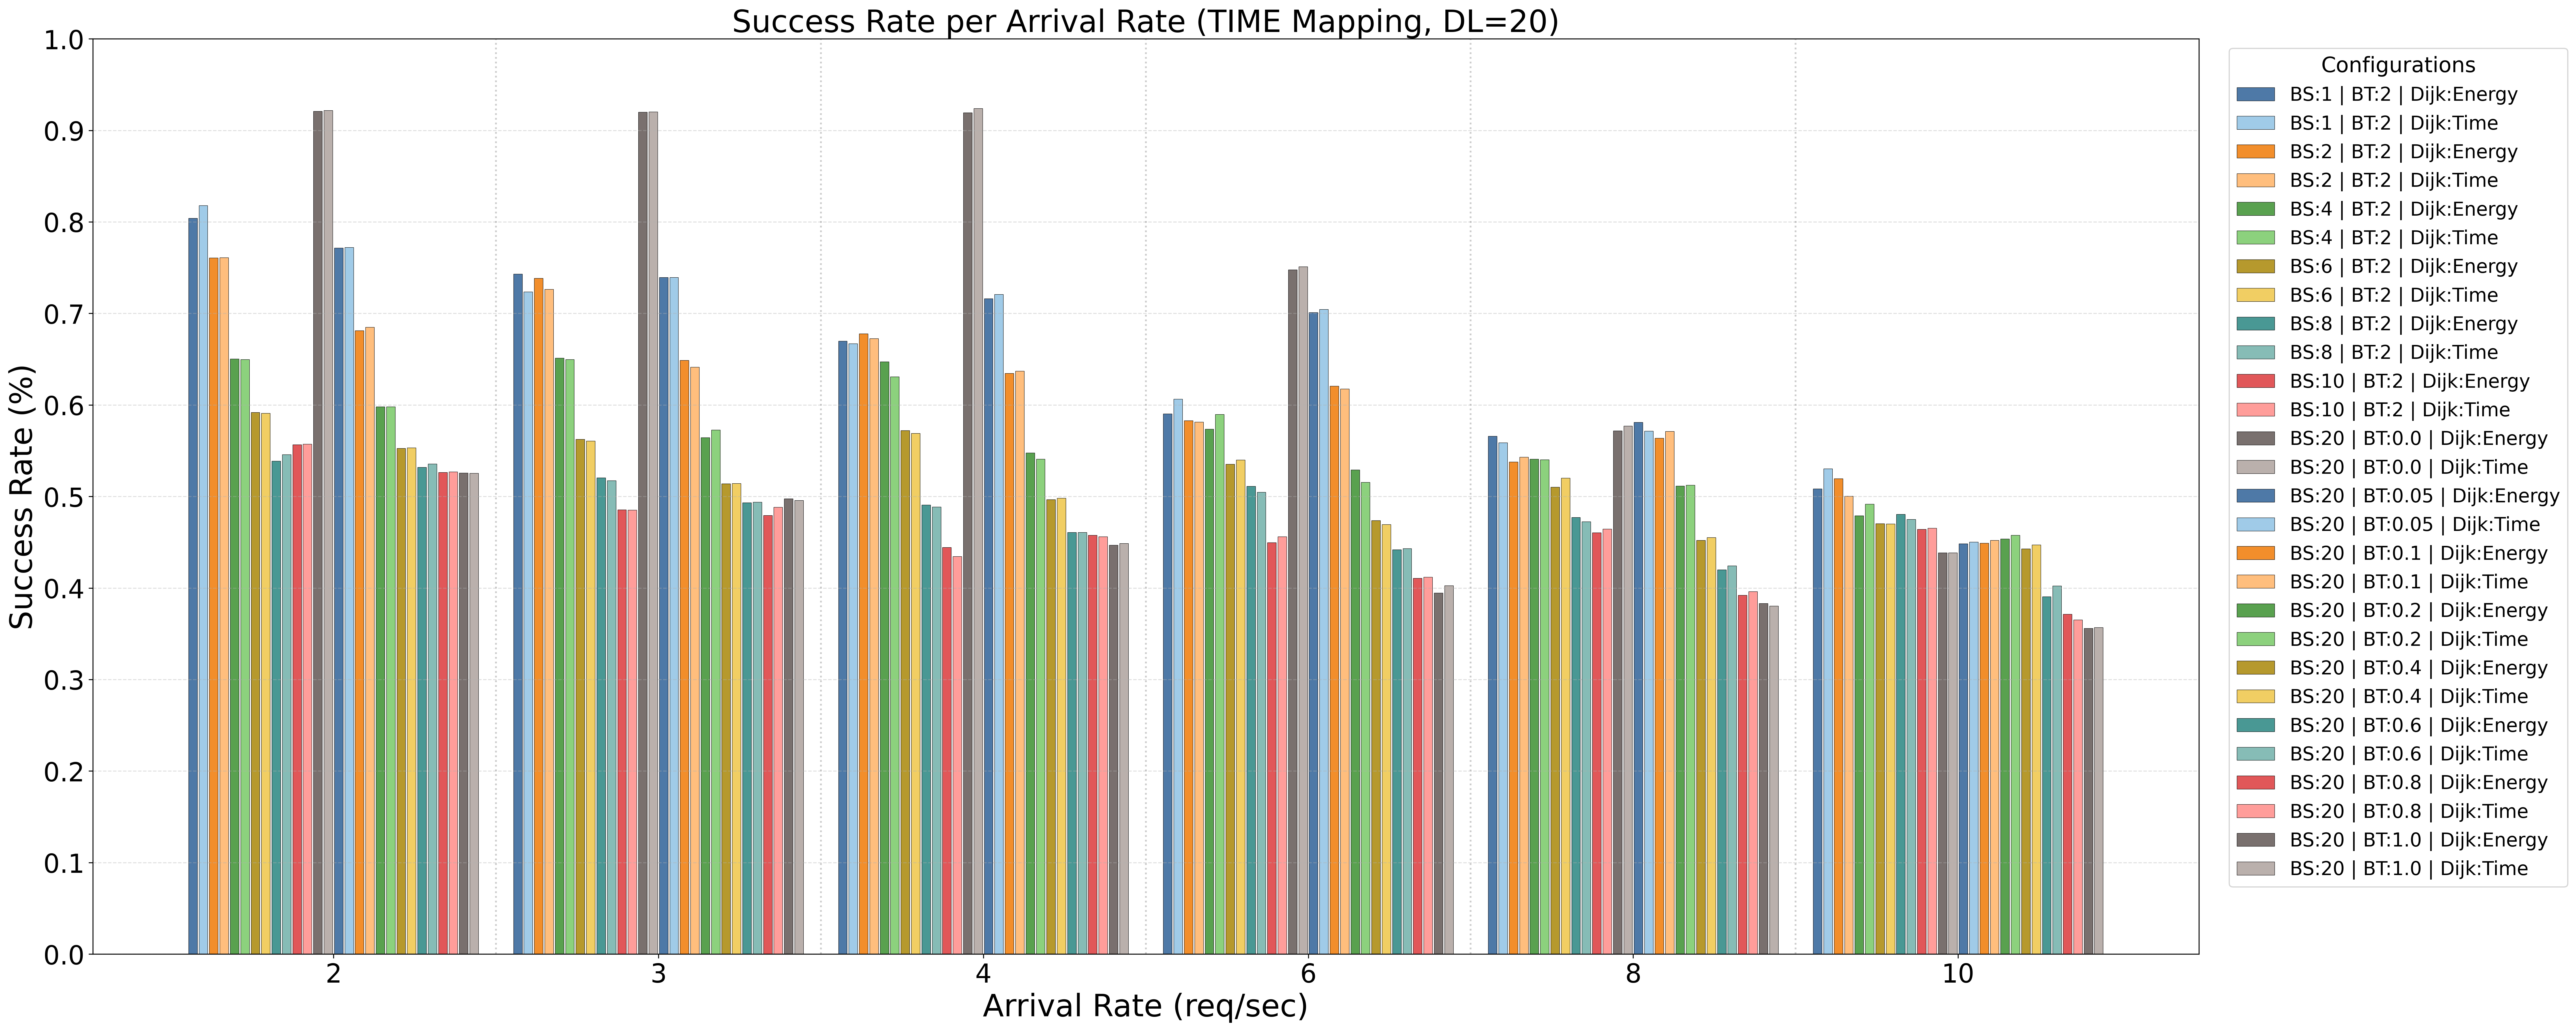
\includegraphics[width=1.3\textwidth]{01_AR_success_rate_time_dl_20.png}}
        \caption{Scomposizione del Success Rate (DL = 20\%).}
        \label{fig:success_rate_time_dl_20}
        \end{figure}

        \begin{figure}[H]
        \makebox[\textwidth][c]{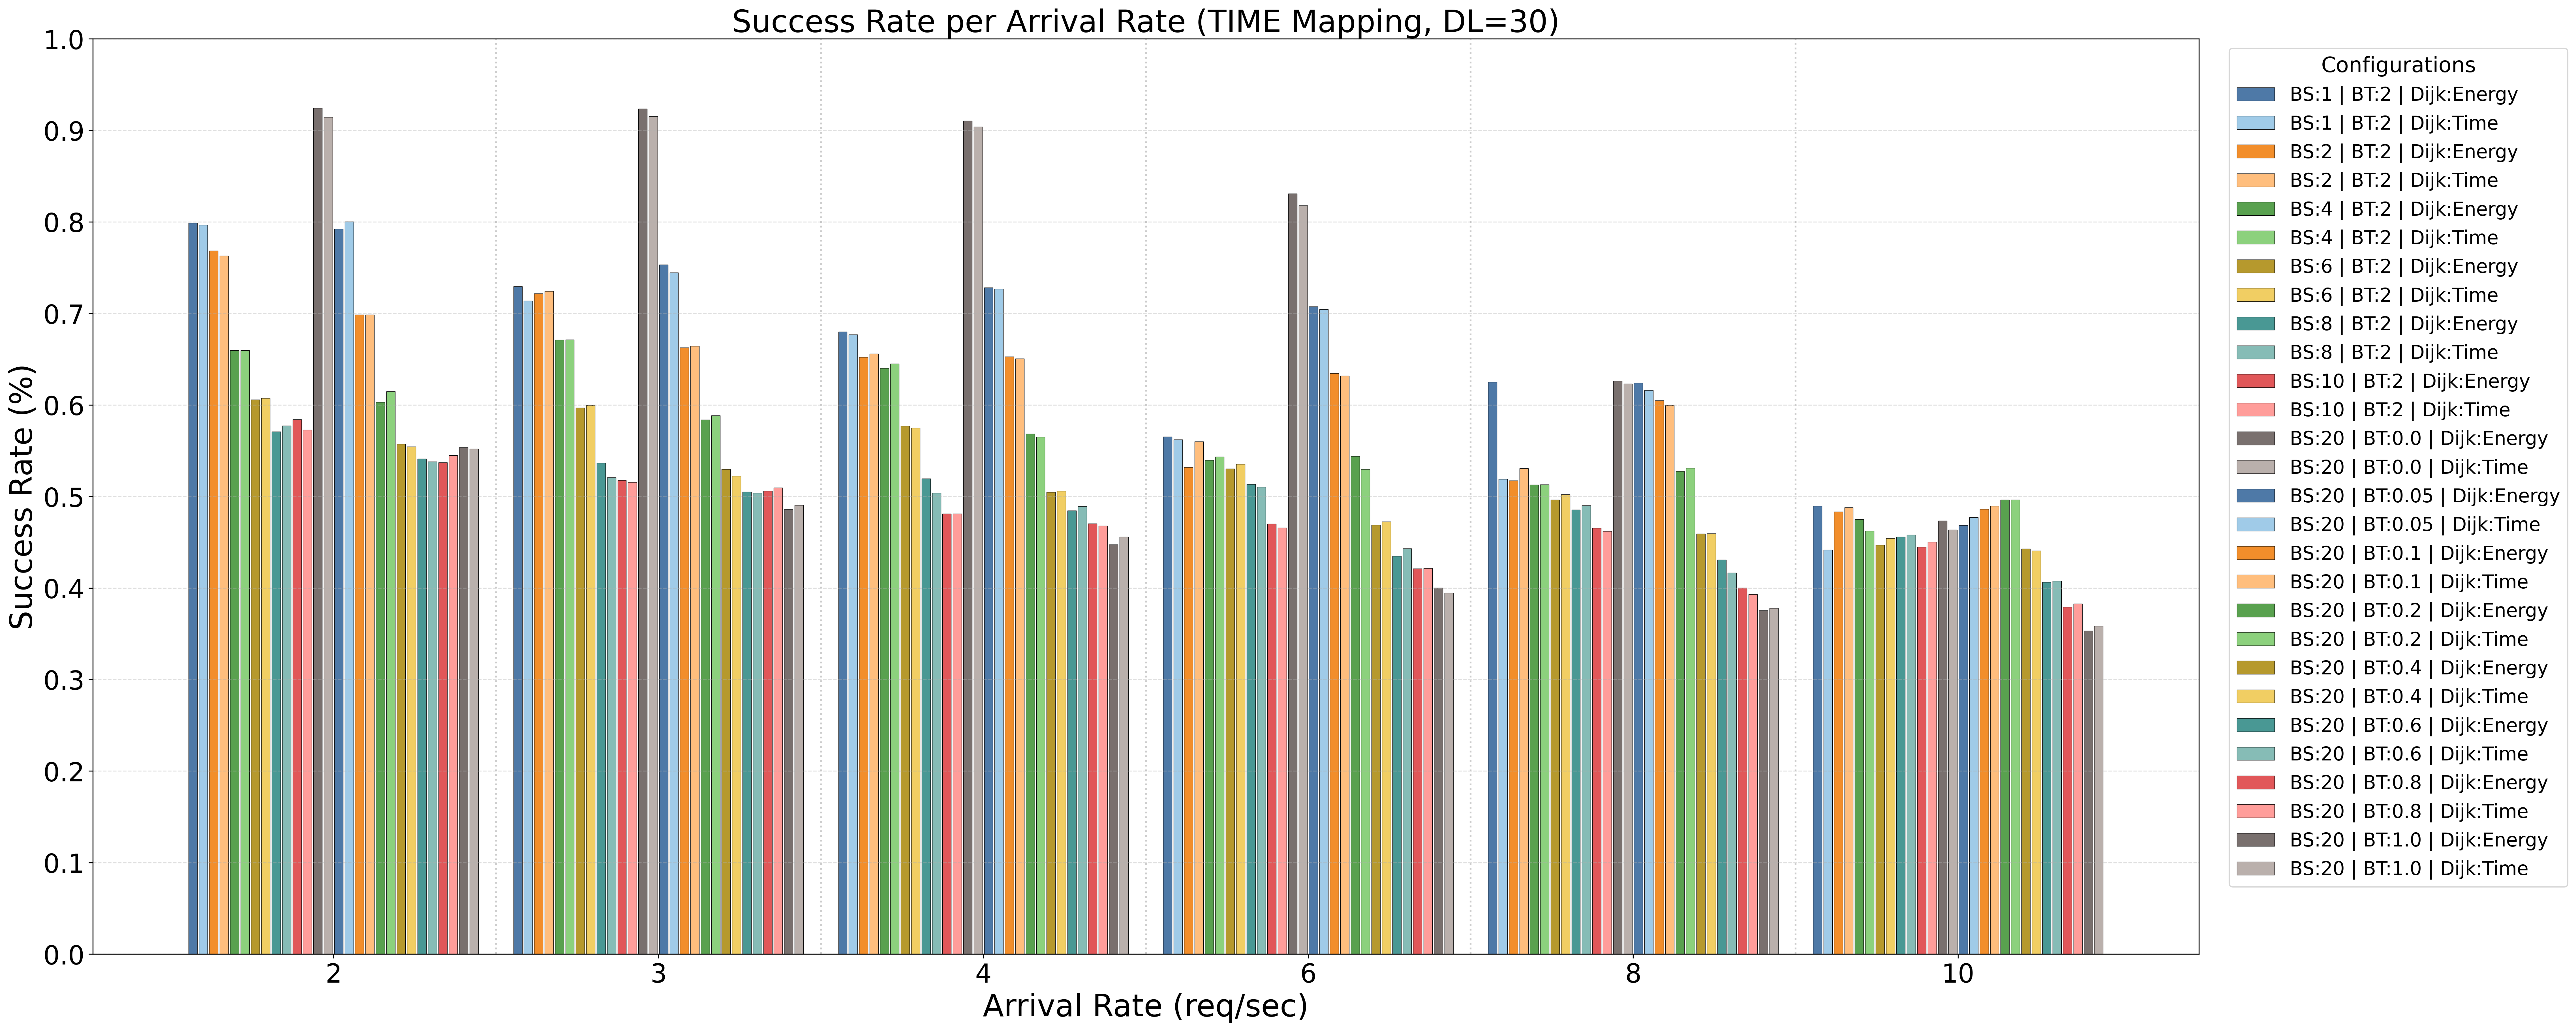
\includegraphics[width=1.3\textwidth]{01_AR_success_rate_time_dl_30.png}}
        \caption{Scomposizione del Success Rate (DL = 30\%).}
        \label{fig:success_rate_time_dl_30}
        \end{figure}


        \subsection{Rejection Reasons}

        \begin{figure}[H]
        \makebox[\textwidth][c]{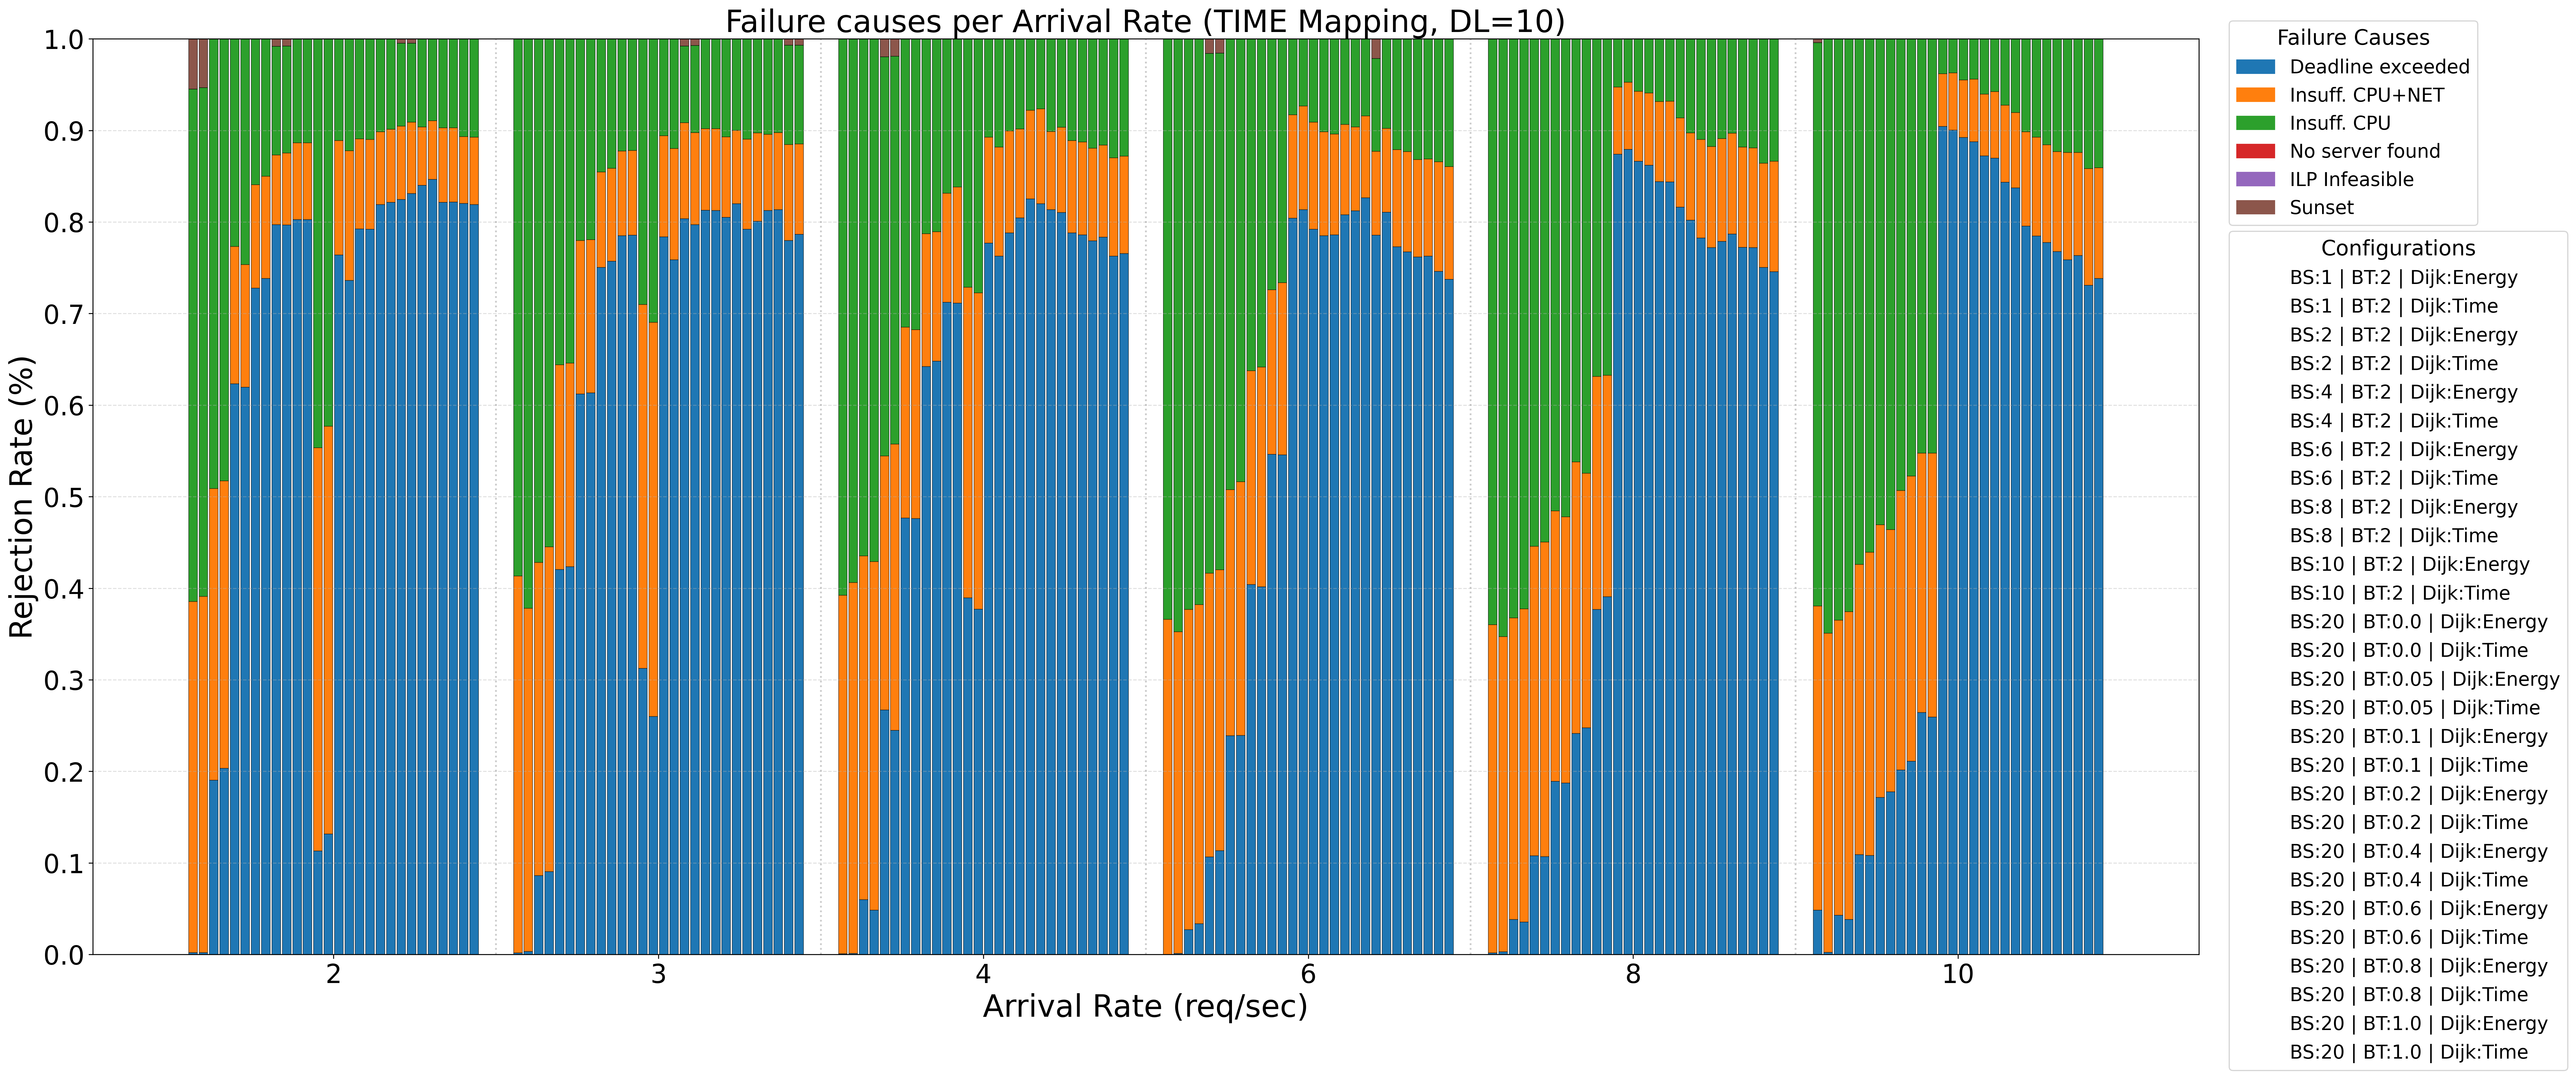
\includegraphics[width=1.3\textwidth]{02_AR_rejection_time_dl_10.png}}
        \caption{Scomposizione del Rejection Reasons (DL = 10\%).}
        \label{fig:rejection_rate_time_dl_10}
        \end{figure}

        \begin{figure}[H]
        \makebox[\textwidth][c]{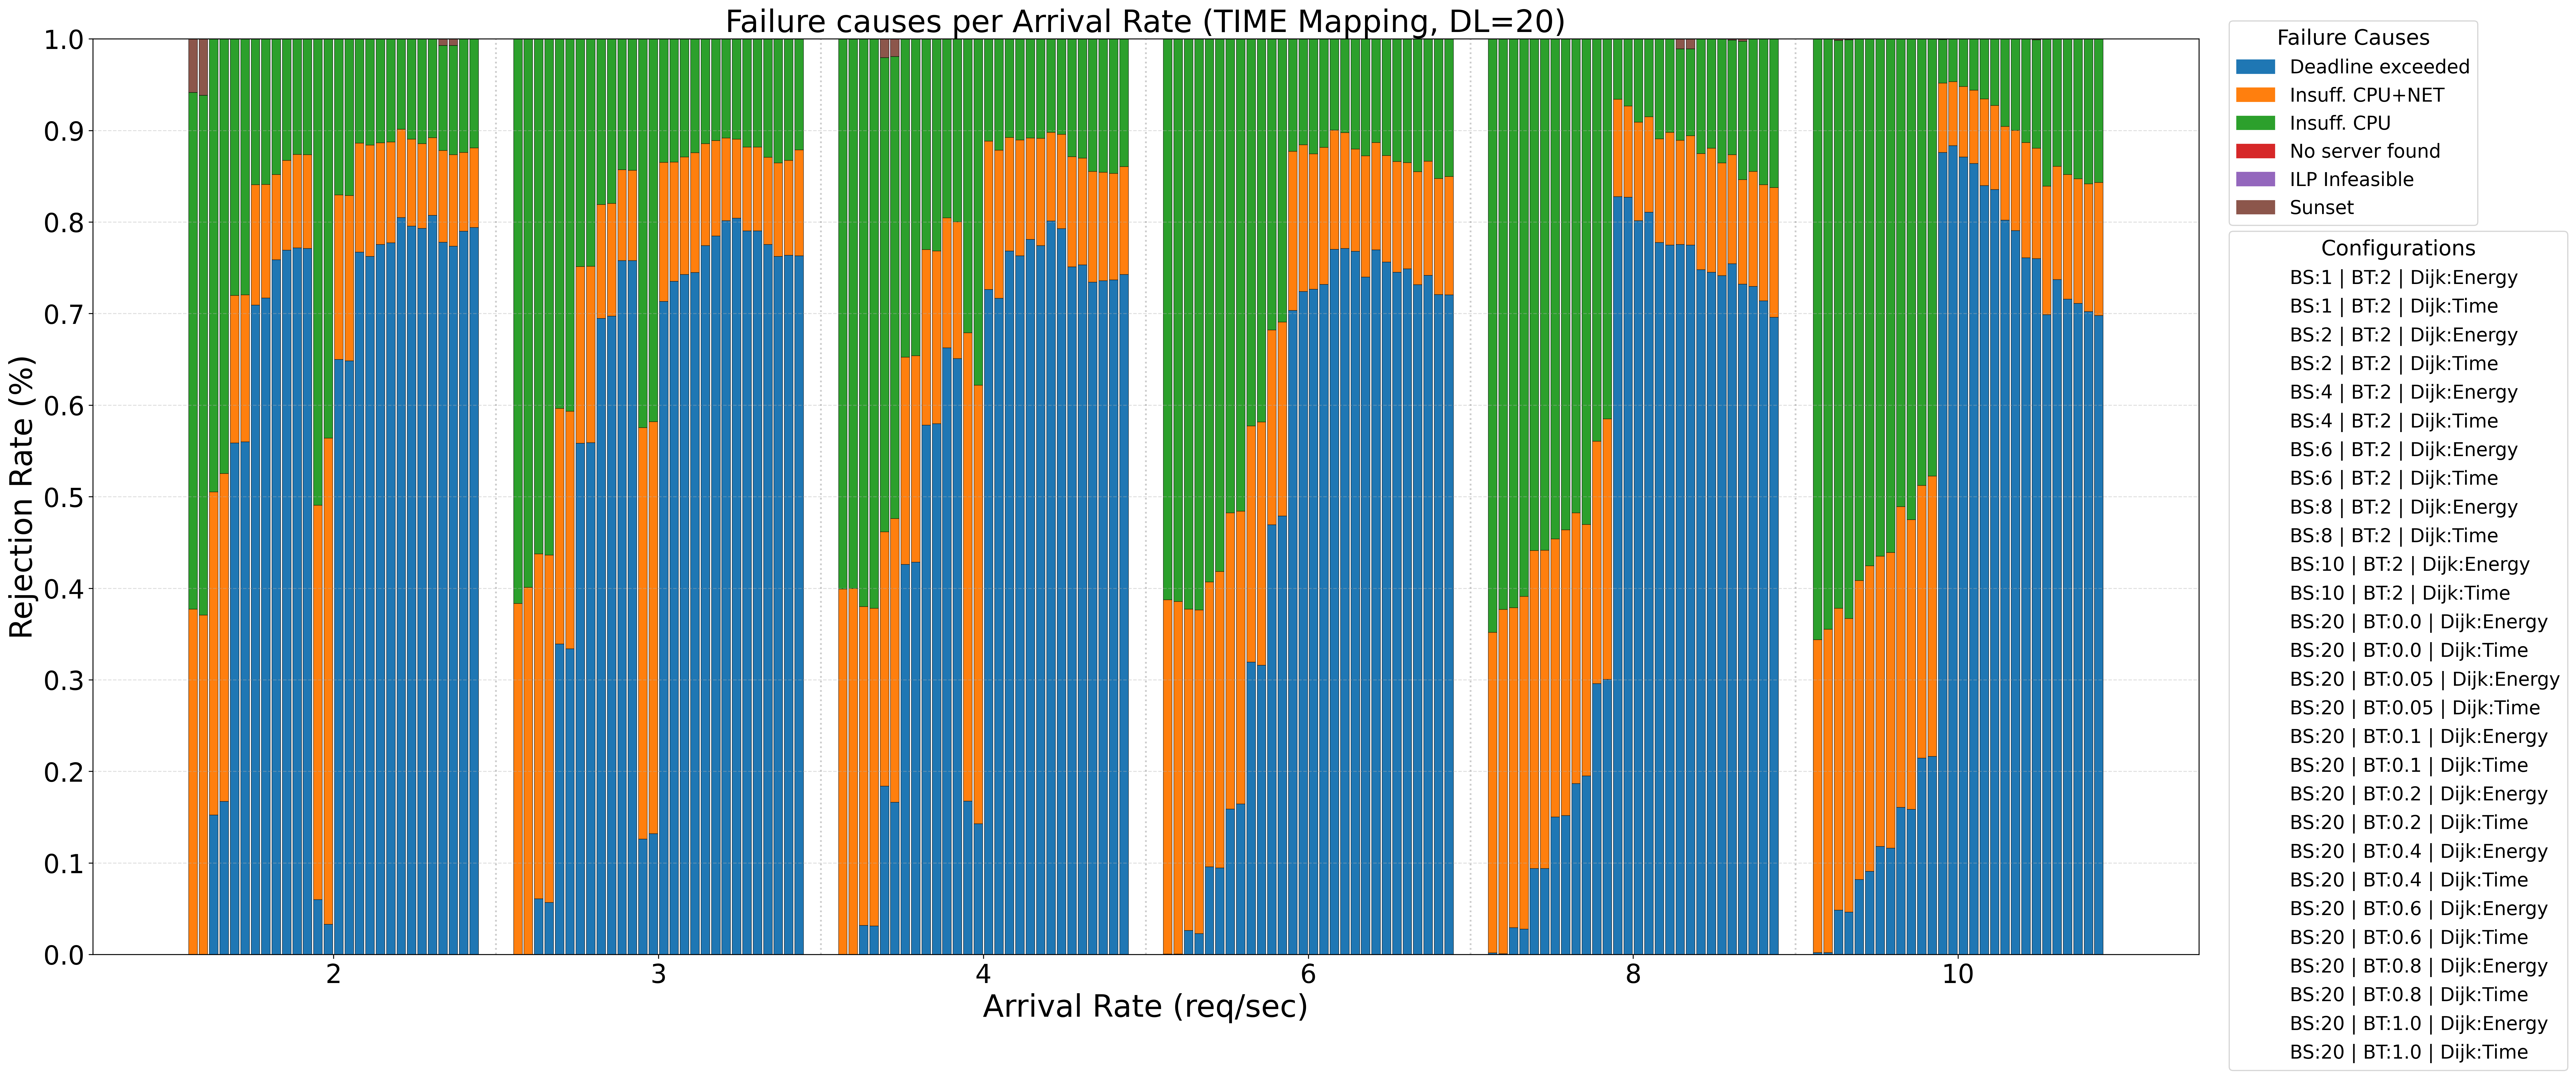
\includegraphics[width=1.3\textwidth]{02_AR_rejection_time_dl_20.png}}
        \caption{Scomposizione del Rejection Reasons (DL = 20\%).}
        \label{fig:rejection_rate_time_dl_20}
        \end{figure}

        \begin{figure}[H]
        \makebox[\textwidth][c]{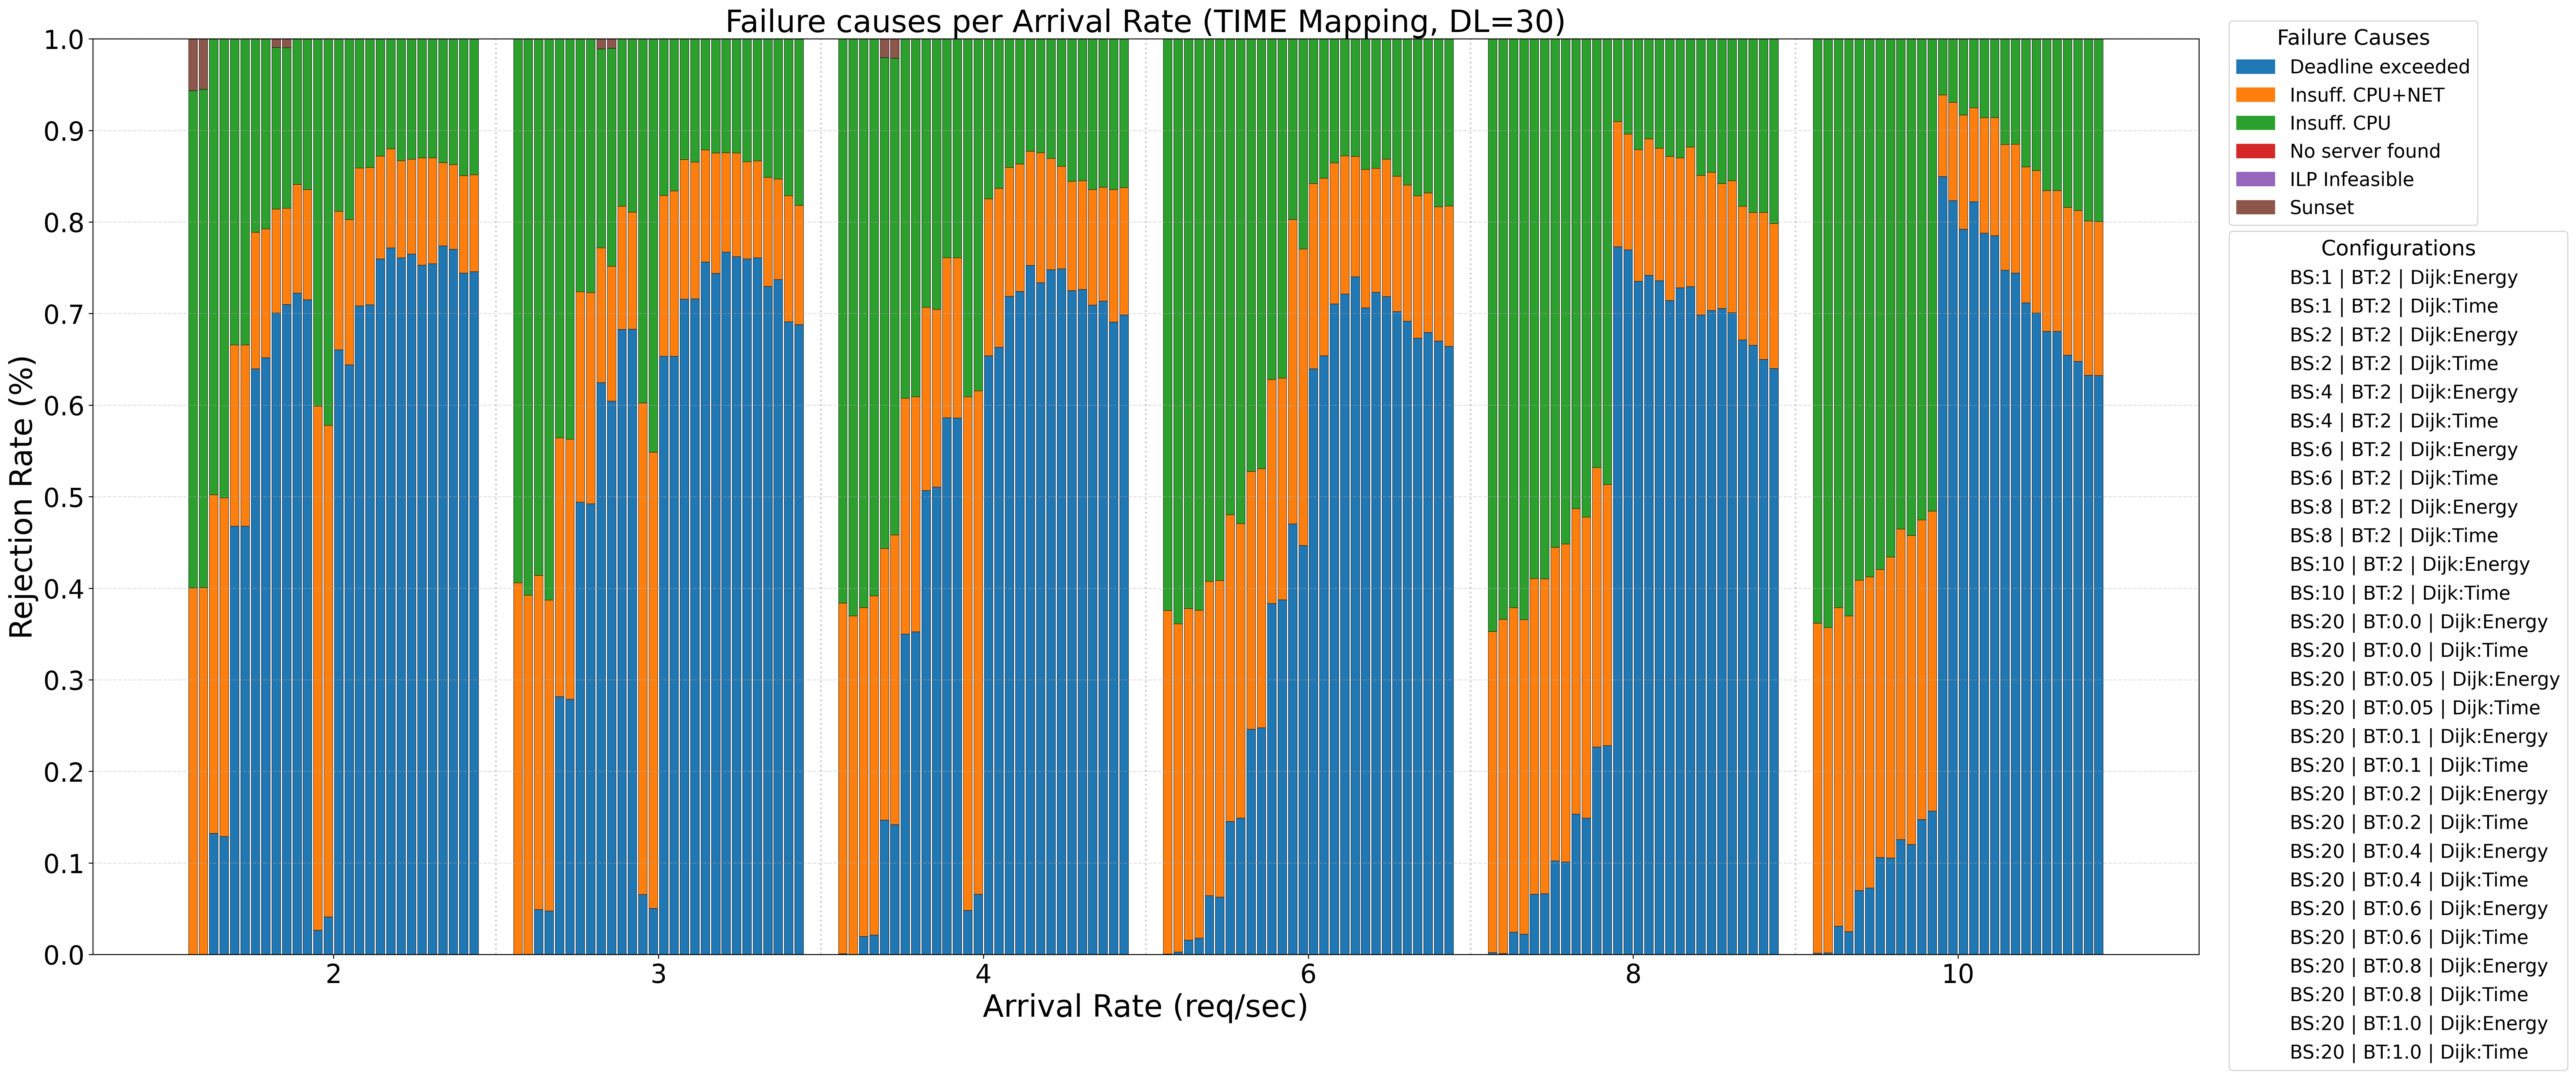
\includegraphics[width=1.3\textwidth]{02_AR_rejection_time_dl_30.png}}
        \caption{Scomposizione del Rejection Reasons (DL = 30\%).}
        \label{fig:rejection_rate_time_dl_30}
        \end{figure}

    \subsection{Response Time}


        \begin{figure}[H]
        \makebox[\textwidth][c]{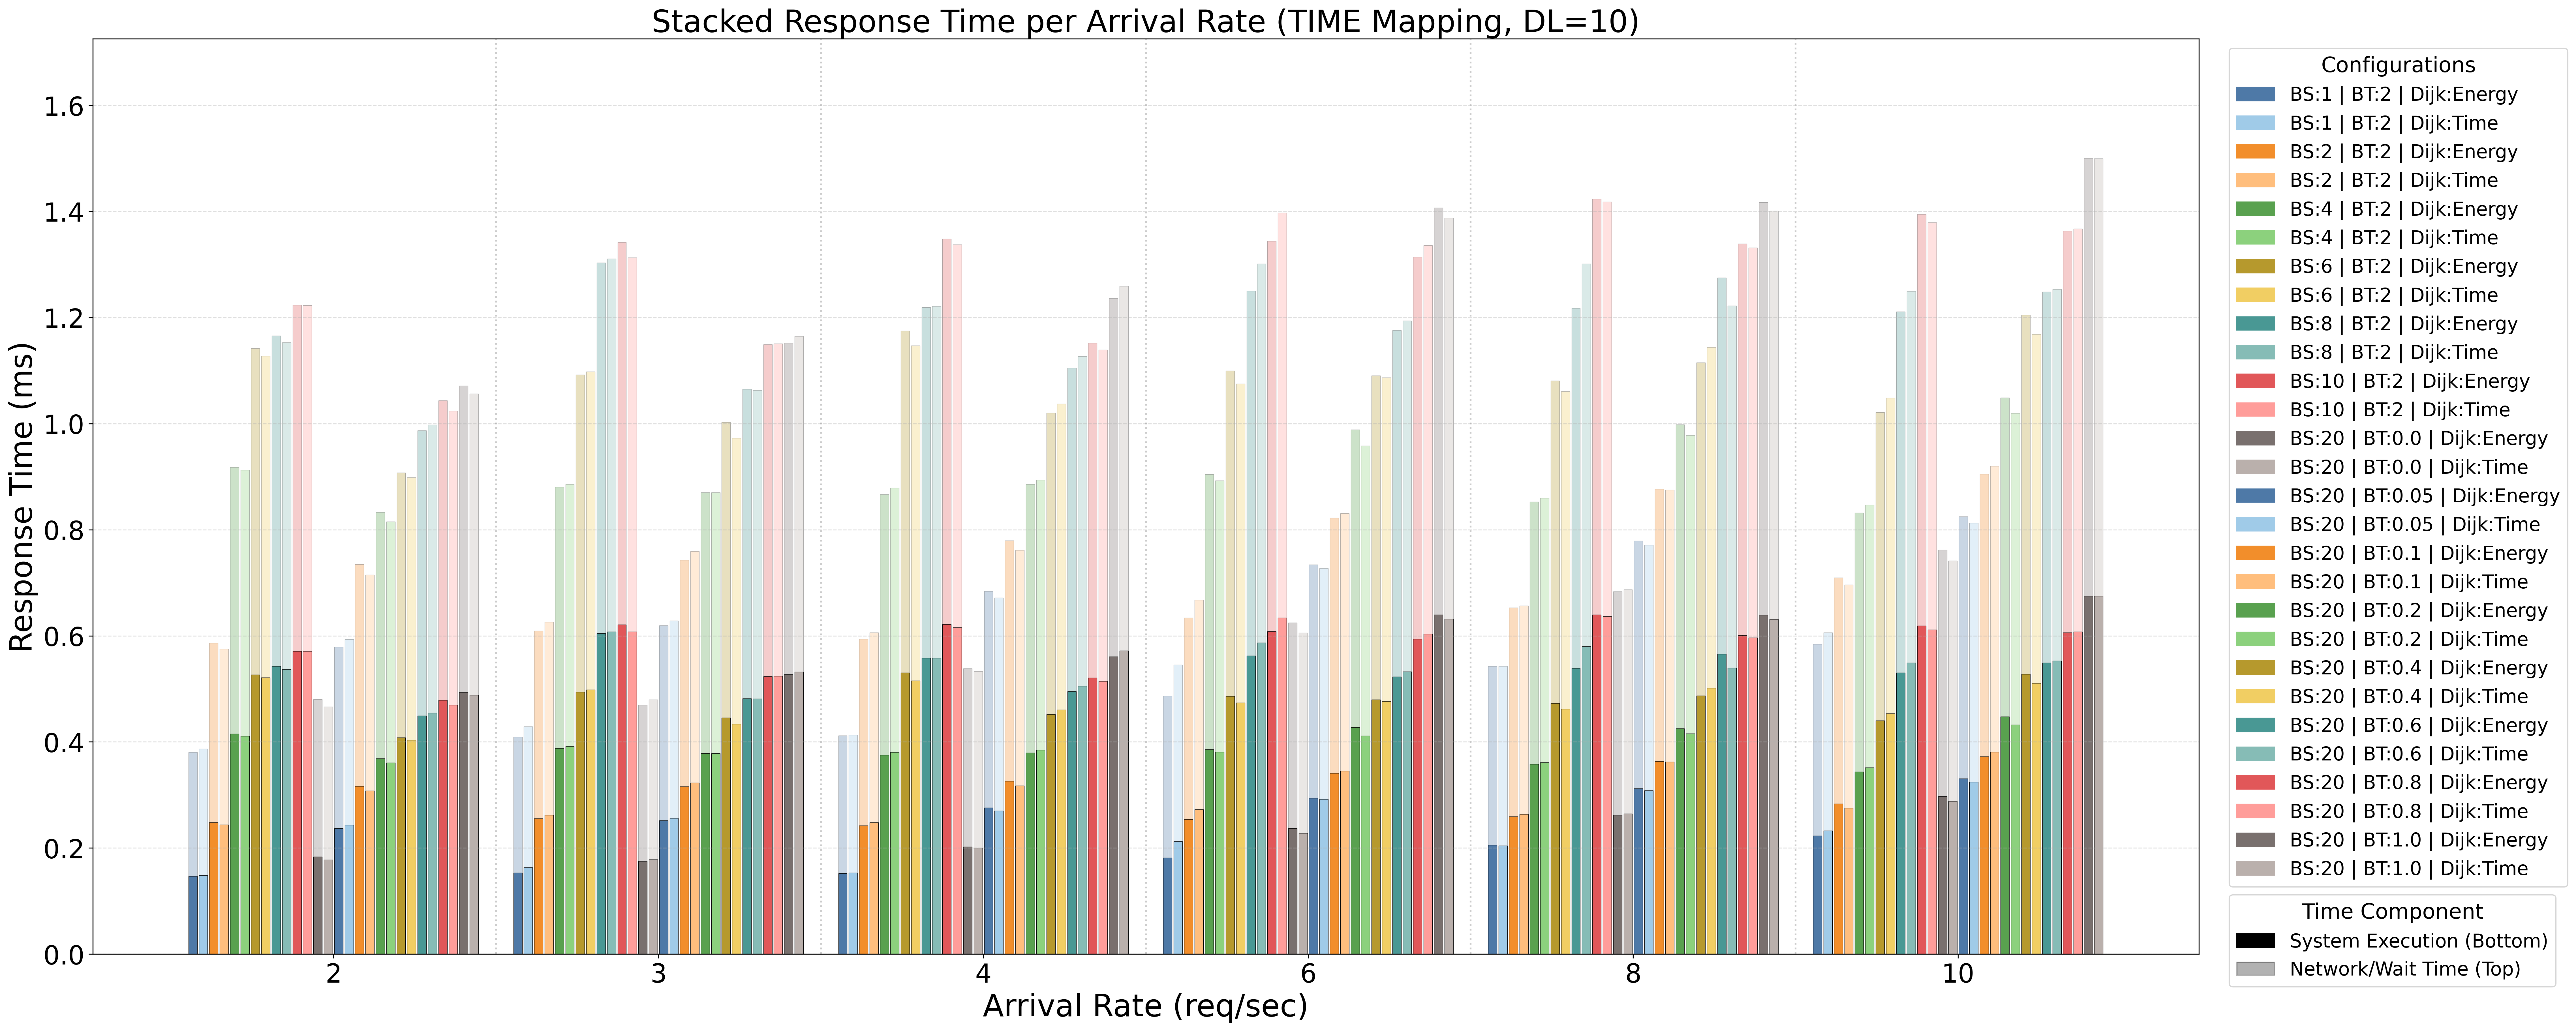
\includegraphics[width=1.3\textwidth]{03_AR_response_time_dl_10.png}}
        \caption{Scomposizione del Response Time (DL = 10\%).}
        \label{fig:response_time_time_dl_10}
        \end{figure}

        \begin{figure}[H]
        \makebox[\textwidth][c]{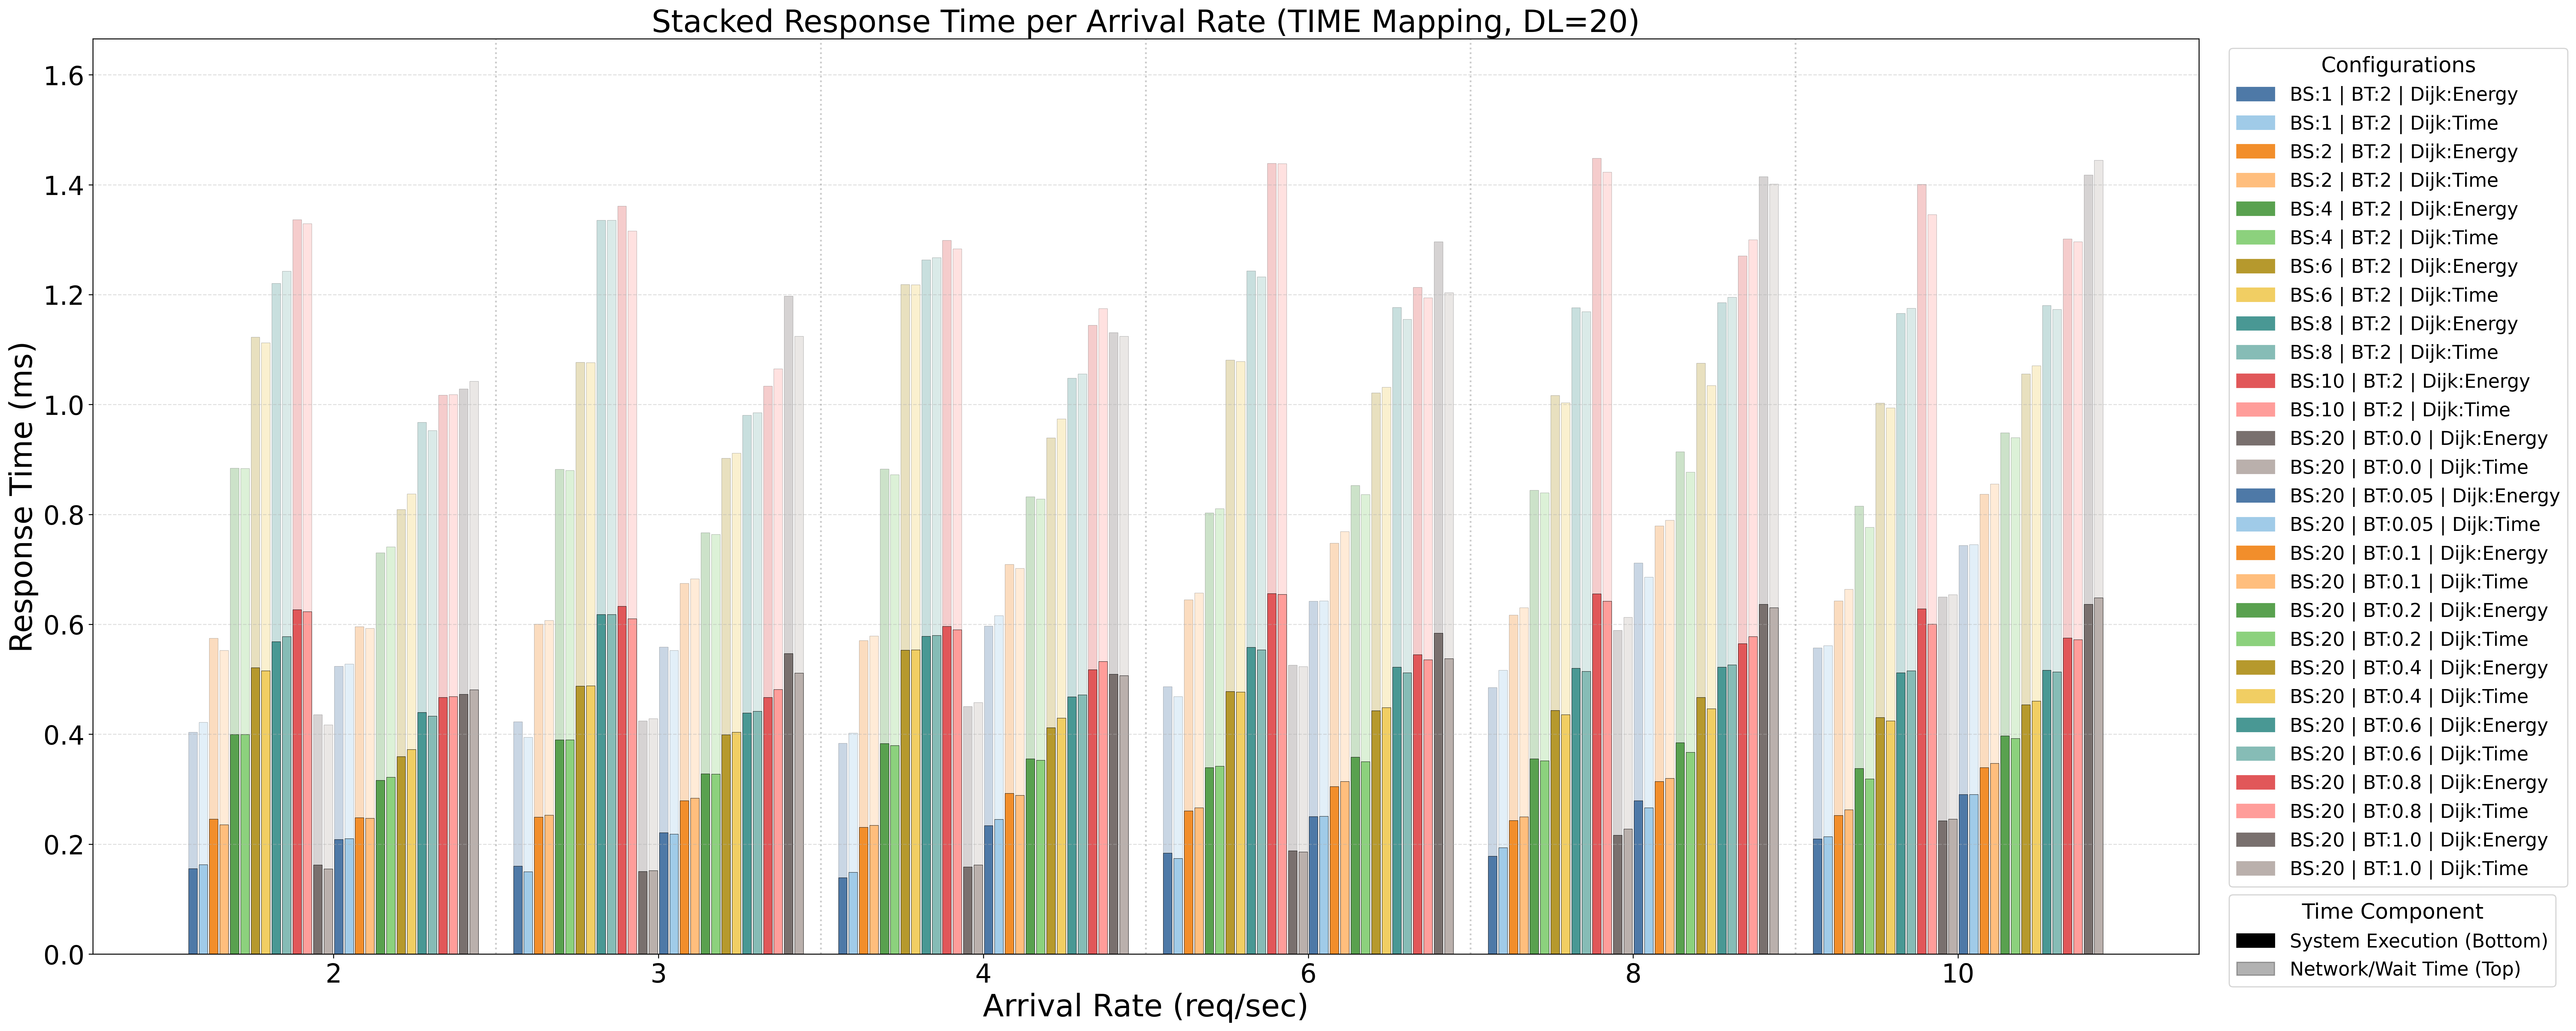
\includegraphics[width=1.3\textwidth]{03_AR_response_time_dl_20.png}}
        \caption{Scomposizione del Response Time (DL = 20\%).}
        \label{fig:response_time_time_dl_20}
        \end{figure}

        \begin{figure}[H]
        \makebox[\textwidth][c]{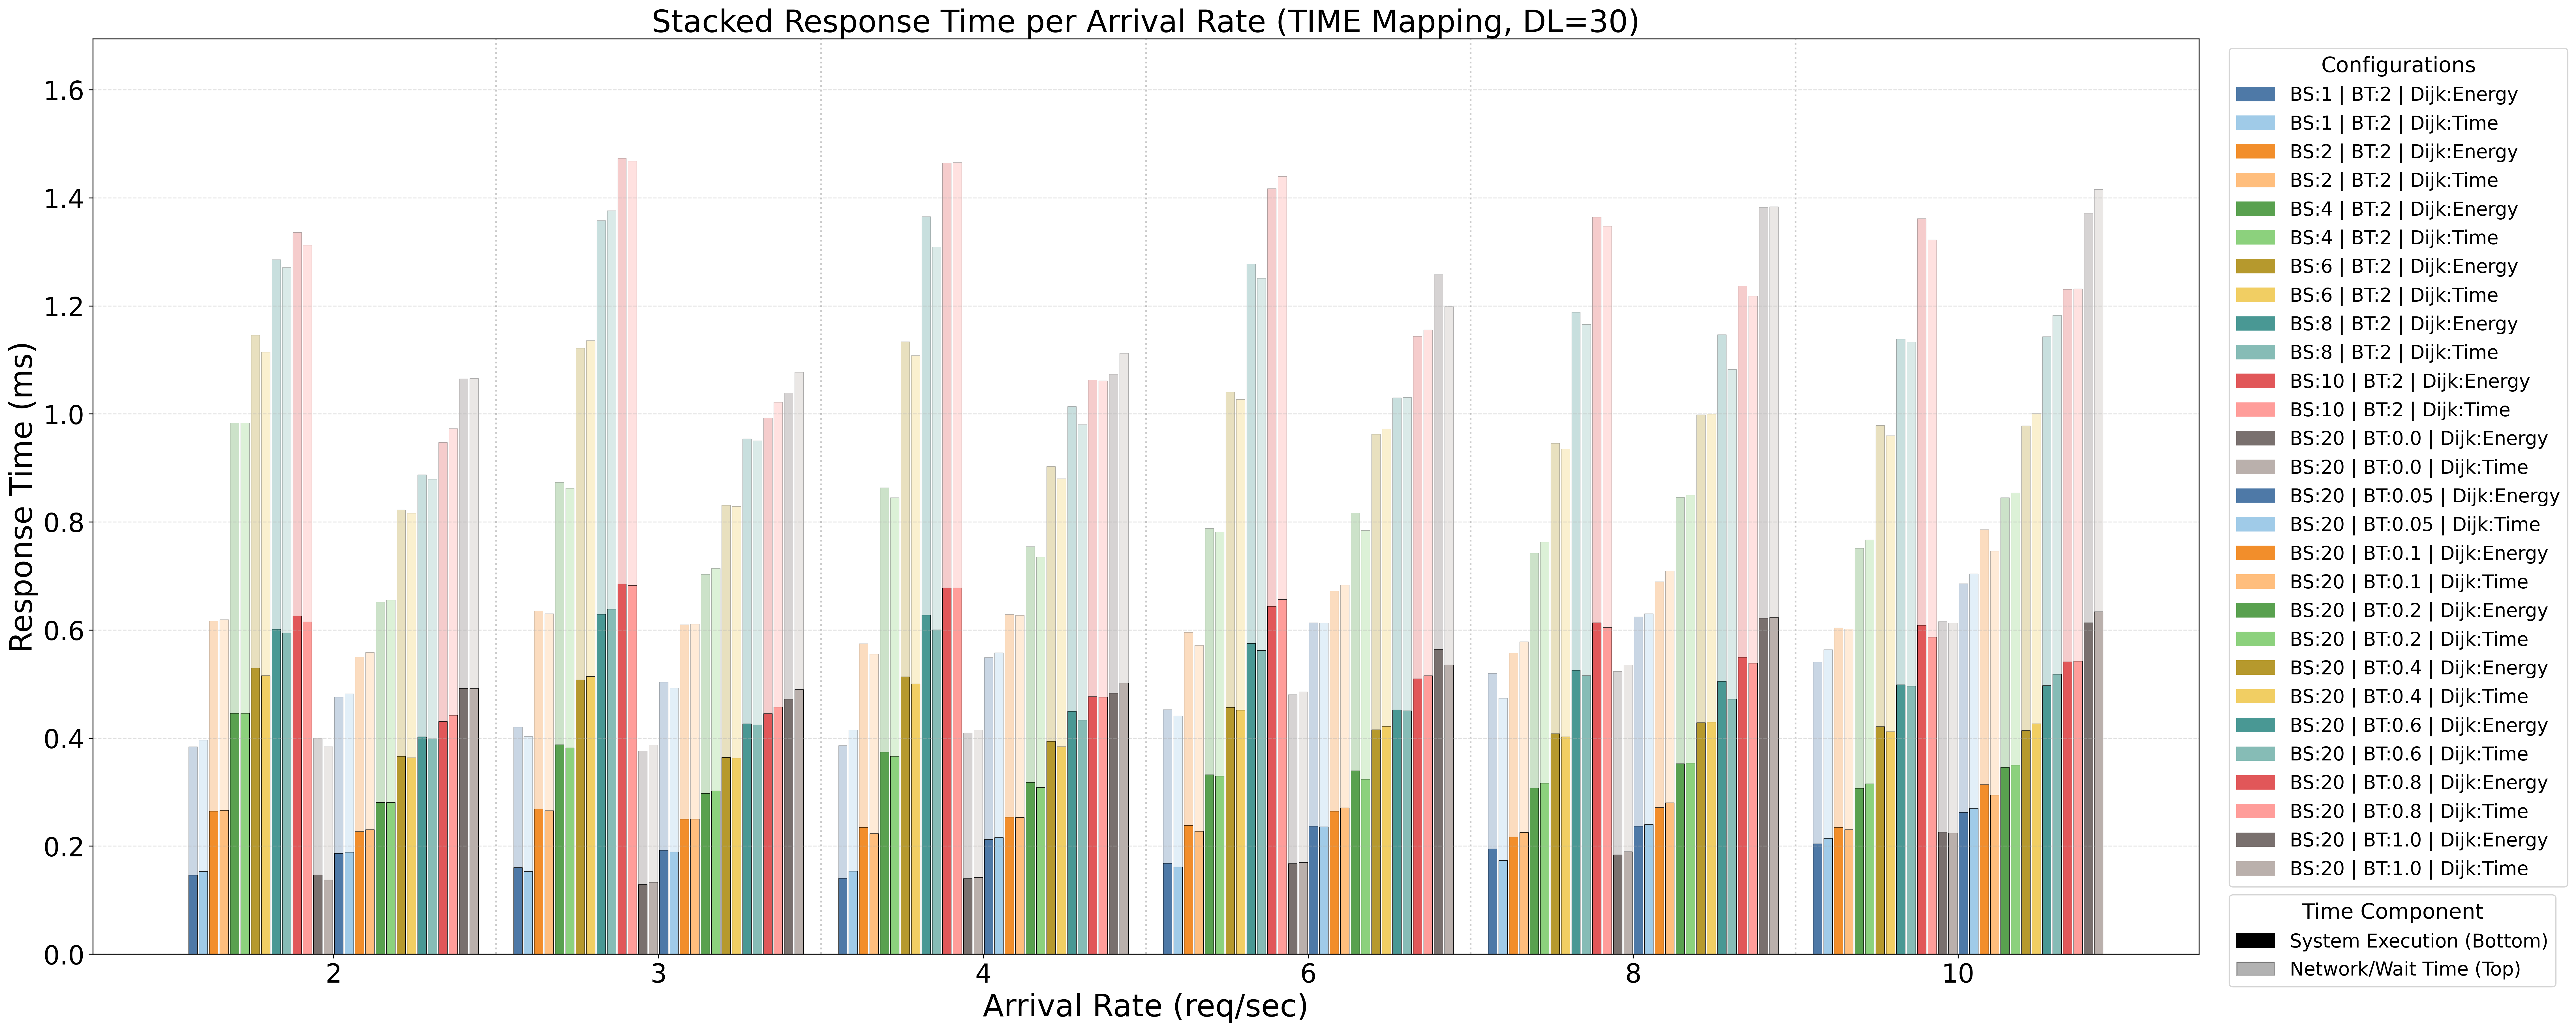
\includegraphics[width=1.3\textwidth]{03_AR_response_time_dl_30.png}}
        \caption{Scomposizione del Response Time (DL = 30\%).}
        \label{fig:response_time_time_dl_30}
        \end{figure}


\section{Dati Sperimentali}

\begin{longtable}{ccccccc}
\caption{Risultati medi aggregati per Deadline, Batch Size (BS), Batch Timeout (BT) e Tasso di Arrivo.}\label{tab:risultati_aggregati_dettagliata} \\
\toprule
\textbf{DL (\%)} & \textbf{BS} & \textbf{BT} & \textbf{Arr. Rate} & \textbf{Succ. Rate} & \textbf{Resp. Time} & \textbf{Exec. Time} \\
& & & (req/sec) & (\%) & (ms) & (ms) \\
\midrule
\endfirsthead

\multicolumn{7}{c}{\tablename\ \thetable\ -- continua dalla pagina precedente} \\
\toprule
\textbf{DL (\%)} & \textbf{BS} & \textbf{BT} & \textbf{Arr. Rate} & \textbf{Succ. Rate} & \textbf{Resp. Time} & \textbf{Exec. Time} \\
& & & (req/sec) & (\%) & (ms) & (ms) \\
\midrule
\endhead

\midrule
\multicolumn{7}{r}{Continua nella pagina successiva...} \\
\endfoot

\bottomrule
\endlastfoot
        10 &  1  &  2.0  & 2 & 73.85 & 0.354 & 0.136 \\
        10 &  1  &  2.0  & 3 & 69.65 & 0.437 & 0.169 \\
        10 &  1  &  2.0  & 4 & 65.13 & 0.446 & 0.171 \\
        10 &  1  &  2.0  & 6 & 57.93 & 0.575 & 0.228 \\
        10 &  1  &  2.0  & 8 & 55.48 & 0.598 & 0.234 \\
        10 &  1  &  2.0  & 10 & 52.83 & 0.637 & 0.249 \\
        \midrule
        10 &  2  &  2.0  & 2 & 71.38 & 0.548 & 0.234 \\
        10 &  2  &  2.0  & 3 & 70.39 & 0.623 & 0.263 \\
        10 &  2  &  2.0  & 4 & 63.37 & 0.617 & 0.256 \\
        10 &  2  &  2.0  & 6 & 54.56 & 0.670 & 0.274 \\
        10 &  2  &  2.0  & 8 & 53.99 & 0.708 & 0.288 \\
        10 &  2  &  2.0  & 10 & 51.66 & 0.738 & 0.298 \\
        \midrule
        10 &  4  &  2.0  & 2 & 58.86 & 0.849 & 0.385 \\
        10 &  4  &  2.0  & 3 & 60.02 & 0.887 & 0.394 \\
        10 &  4  &  2.0  & 4 & 58.61 & 0.900 & 0.394 \\
        10 &  4  &  2.0  & 6 & 53.29 & 0.911 & 0.393 \\
        10 &  4  &  2.0  & 8 & 50.94 & 0.913 & 0.390 \\
        10 &  4  &  2.0  & 10 & 48.36 & 0.890 & 0.374 \\
        \midrule
        10 &  6  &  2.0  & 2 & 52.16 & 1.059 & 0.491 \\
        10 &  6  &  2.0  & 3 & 51.36 & 1.032 & 0.469 \\
        10 &  6  &  2.0  & 4 & 50.51 & 1.117 & 0.506 \\
        10 &  6  &  2.0  & 6 & 50.48 & 1.090 & 0.486 \\
        10 &  6  &  2.0  & 8 & 48.72 & 1.066 & 0.467 \\
        10 &  6  &  2.0  & 10 & 46.43 & 1.024 & 0.444 \\
        \midrule
        10 &  8  &  2.0  & 2 & 49.62 & 1.096 & 0.510 \\
        10 &  8  &  2.0  & 3 & 46.19 & 1.178 & 0.544 \\
        10 &  8  &  2.0  & 4 & 45.18 & 1.167 & 0.533 \\
        10 &  8  &  2.0  & 6 & 47.81 & 1.282 & 0.577 \\
        10 &  8  &  2.0  & 8 & 47.81 & 1.241 & 0.551 \\
        10 &  8  &  2.0  & 10 & 47.27 & 1.210 & 0.531 \\
        \midrule
        10 &  10  &  2.0  & 2 & 49.36 & 1.139 & 0.532 \\
        10 &  10  &  2.0  & 3 & 43.04 & 1.198 & 0.553 \\
        10 &  10  &  2.0  & 4 & 41.24 & 1.272 & 0.585 \\
        10 &  10  &  2.0  & 6 & 42.22 & 1.385 & 0.629 \\
        10 &  10  &  2.0  & 8 & 44.20 & 1.428 & 0.641 \\
        10 &  10  &  2.0  & 10 & 46.06 & 1.383 & 0.612 \\
        \midrule
        10 &  20  &  0.0  & 2 & 93.80 & 0.469 & 0.179 \\
        10 &  20  &  0.0  & 3 & 91.84 & 0.483 & 0.181 \\
        10 &  20  &  0.0  & 4 & 89.37 & 0.536 & 0.201 \\
        10 &  20  &  0.0  & 6 & 67.61 & 0.621 & 0.235 \\
        10 &  20  &  0.0  & 8 & 53.35 & 0.682 & 0.262 \\
        10 &  20  &  0.0  & 10 & 41.88 & 0.747 & 0.291 \\
        \midrule
        10 &  20  &  0.05  & 2 & 76.38 & 0.591 & 0.242 \\
        10 &  20  &  0.05  & 3 & 72.90 & 0.613 & 0.248 \\
        10 &  20  &  0.05  & 4 & 71.45 & 0.678 & 0.273 \\
        10 &  20  &  0.05  & 6 & 67.14 & 0.730 & 0.293 \\
        10 &  20  &  0.05  & 8 & 54.39 & 0.775 & 0.310 \\
        10 &  20  &  0.05  & 10 & 41.66 & 0.824 & 0.330 \\
        \midrule
        10 &  20  &  0.1  & 2 & 66.39 & 0.707 & 0.301 \\
        10 &  20  &  0.1  & 3 & 63.75 & 0.745 & 0.315 \\
        10 &  20  &  0.1  & 4 & 62.32 & 0.776 & 0.325 \\
        10 &  20  &  0.1  & 6 & 59.83 & 0.831 & 0.345 \\
        10 &  20  &  0.1  & 8 & 52.82 & 0.872 & 0.361 \\
        10 &  20  &  0.1  & 10 & 41.95 & 0.907 & 0.374 \\
        \midrule
        10 &  20  &  0.2  & 2 & 58.08 & 0.798 & 0.352 \\
        10 &  20  &  0.2  & 3 & 55.17 & 0.863 & 0.376 \\
        10 &  20  &  0.2  & 4 & 53.94 & 0.898 & 0.388 \\
        10 &  20  &  0.2  & 6 & 51.34 & 0.964 & 0.414 \\
        10 &  20  &  0.2  & 8 & 50.06 & 0.984 & 0.419 \\
        10 &  20  &  0.2  & 10 & 42.28 & 1.032 & 0.439 \\
        \midrule
        10 &  20  &  0.4  & 2 & 53.26 & 0.899 & 0.405 \\
        10 &  20  &  0.4  & 3 & 49.12 & 0.966 & 0.431 \\
        10 &  20  &  0.4  & 4 & 48.25 & 1.021 & 0.453 \\
        10 &  20  &  0.4  & 6 & 45.52 & 1.090 & 0.478 \\
        10 &  20  &  0.4  & 8 & 44.11 & 1.126 & 0.493 \\
        10 &  20  &  0.4  & 10 & 42.32 & 1.185 & 0.518 \\
        \midrule
        10 &  20  &  0.6  & 2 & 51.64 & 0.972 & 0.443 \\
        10 &  20  &  0.6  & 3 & 47.25 & 1.037 & 0.469 \\
        10 &  20  &  0.6  & 4 & 44.83 & 1.113 & 0.500 \\
        10 &  20  &  0.6  & 6 & 42.27 & 1.185 & 0.527 \\
        10 &  20  &  0.6  & 8 & 40.69 & 1.237 & 0.547 \\
        10 &  20  &  0.6  & 10 & 39.01 & 1.241 & 0.546 \\
        \midrule
        10 &  20  &  0.8  & 2 & 49.63 & 0.997 & 0.458 \\
        10 &  20  &  0.8  & 3 & 46.74 & 1.108 & 0.504 \\
        10 &  20  &  0.8  & 4 & 43.65 & 1.152 & 0.521 \\
        10 &  20  &  0.8  & 6 & 39.61 & 1.303 & 0.587 \\
        10 &  20  &  0.8  & 8 & 38.11 & 1.305 & 0.583 \\
        10 &  20  &  0.8  & 10 & 37.10 & 1.333 & 0.591 \\
        \midrule
        10 &  20  &  1.0  & 2 & 48.68 & 1.016 & 0.468 \\
        10 &  20  &  1.0  & 3 & 45.88 & 1.153 & 0.528 \\
        10 &  20  &  1.0  & 4 & 41.71 & 1.237 & 0.564 \\
        10 &  20  &  1.0  & 6 & 38.01 & 1.373 & 0.623 \\
        10 &  20  &  1.0  & 8 & 36.55 & 1.389 & 0.624 \\
        10 &  20  &  1.0  & 10 & 34.94 & 1.450 & 0.650 \\
        \midrule
        \midrule
        20 &  1  &  2.0  & 2 & 73.92 & 0.347 & 0.132 \\
        20 &  1  &  2.0  & 3 & 67.25 & 0.411 & 0.159 \\
        20 &  1  &  2.0  & 4 & 61.20 & 0.410 & 0.155 \\
        20 &  1  &  2.0  & 6 & 55.43 & 0.498 & 0.190 \\
        20 &  1  &  2.0  & 8 & 56.13 & 0.538 & 0.205 \\
        20 &  1  &  2.0  & 10 & 49.66 & 0.579 & 0.222 \\
        \midrule
        20 &  2  &  2.0  & 2 & 71.26 & 0.537 & 0.231 \\
        20 &  2  &  2.0  & 3 & 67.32 & 0.567 & 0.236 \\
        20 &  2  &  2.0  & 4 & 61.38 & 0.568 & 0.234 \\
        20 &  2  &  2.0  & 6 & 53.69 & 0.644 & 0.262 \\
        20 &  2  &  2.0  & 8 & 49.91 & 0.657 & 0.265 \\
        20 &  2  &  2.0  & 10 & 47.51 & 0.675 & 0.270 \\
        \midrule
        20 &  4  &  2.0  & 2 & 60.47 & 0.834 & 0.378 \\
        20 &  4  &  2.0  & 3 & 59.60 & 0.834 & 0.371 \\
        20 &  4  &  2.0  & 4 & 56.83 & 0.864 & 0.380 \\
        20 &  4  &  2.0  & 6 & 52.10 & 0.856 & 0.366 \\
        20 &  4  &  2.0  & 8 & 48.81 & 0.854 & 0.361 \\
        20 &  4  &  2.0  & 10 & 45.05 & 0.827 & 0.344 \\
        \midrule
        20 &  6  &  2.0  & 2 & 54.38 & 1.015 & 0.471 \\
        20 &  6  &  2.0  & 3 & 52.79 & 1.027 & 0.467 \\
        20 &  6  &  2.0  & 4 & 51.88 & 1.095 & 0.496 \\
        20 &  6  &  2.0  & 6 & 49.55 & 1.028 & 0.455 \\
        20 &  6  &  2.0  & 8 & 47.48 & 1.011 & 0.443 \\
        20 &  6  &  2.0  & 10 & 43.86 & 0.974 & 0.418 \\
        \midrule
        20 &  8  &  2.0  & 2 & 50.41 & 1.106 & 0.515 \\
        20 &  8  &  2.0  & 3 & 47.84 & 1.159 & 0.534 \\
        20 &  8  &  2.0  & 4 & 46.24 & 1.196 & 0.547 \\
        20 &  8  &  2.0  & 6 & 46.86 & 1.238 & 0.557 \\
        20 &  8  &  2.0  & 8 & 45.50 & 1.169 & 0.517 \\
        20 &  8  &  2.0  & 10 & 45.20 & 1.149 & 0.503 \\
        \midrule
        20 &  10  &  2.0  & 2 & 51.41 & 1.184 & 0.554 \\
        20 &  10  &  2.0  & 3 & 44.67 & 1.255 & 0.582 \\
        20 &  10  &  2.0  & 4 & 42.07 & 1.308 & 0.603 \\
        20 &  10  &  2.0  & 6 & 42.60 & 1.413 & 0.644 \\
        20 &  10  &  2.0  & 8 & 44.37 & 1.385 & 0.623 \\
        20 &  10  &  2.0  & 10 & 43.83 & 1.338 & 0.595 \\
        \midrule
        20 &  20  &  0.0  & 2 & 93.18 & 0.408 & 0.149 \\
        20 &  20  &  0.0  & 3 & 92.22 & 0.424 & 0.150 \\
        20 &  20  &  0.0  & 4 & 91.42 & 0.449 & 0.158 \\
        20 &  20  &  0.0  & 6 & 75.48 & 0.524 & 0.187 \\
        20 &  20  &  0.0  & 8 & 57.08 & 0.589 & 0.216 \\
        20 &  20  &  0.0  & 10 & 43.94 & 0.646 & 0.241 \\
        \midrule
        20 &  20  &  0.05  & 2 & 77.31 & 0.518 & 0.206 \\
        20 &  20  &  0.05  & 3 & 73.65 & 0.553 & 0.219 \\
        20 &  20  &  0.05  & 4 & 72.22 & 0.597 & 0.235 \\
        20 &  20  &  0.05  & 6 & 69.61 & 0.641 & 0.250 \\
        20 &  20  &  0.05  & 8 & 57.28 & 0.695 & 0.271 \\
        20 &  20  &  0.05  & 10 & 44.91 & 0.745 & 0.291 \\
        \midrule
        20 &  20  &  0.1  & 2 & 68.22 & 0.602 & 0.251 \\
        20 &  20  &  0.1  & 3 & 65.10 & 0.650 & 0.268 \\
        20 &  20  &  0.1  & 4 & 63.26 & 0.688 & 0.282 \\
        20 &  20  &  0.1  & 6 & 60.88 & 0.750 & 0.304 \\
        20 &  20  &  0.1  & 8 & 56.31 & 0.774 & 0.312 \\
        20 &  20  &  0.1  & 10 & 44.90 & 0.831 & 0.336 \\
        \midrule
        20 &  20  &  0.2  & 2 & 59.23 & 0.719 & 0.314 \\
        20 &  20  &  0.2  & 3 & 56.47 & 0.758 & 0.325 \\
        20 &  20  &  0.2  & 4 & 54.13 & 0.802 & 0.341 \\
        20 &  20  &  0.2  & 6 & 51.61 & 0.854 & 0.359 \\
        20 &  20  &  0.2  & 8 & 51.20 & 0.890 & 0.373 \\
        20 &  20  &  0.2  & 10 & 45.44 & 0.939 & 0.392 \\
        \midrule
        20 &  20  &  0.4  & 2 & 53.56 & 0.807 & 0.359 \\
        20 &  20  &  0.4  & 3 & 50.22 & 0.898 & 0.397 \\
        20 &  20  &  0.4  & 4 & 48.30 & 0.946 & 0.416 \\
        20 &  20  &  0.4  & 6 & 46.47 & 1.028 & 0.447 \\
        20 &  20  &  0.4  & 8 & 45.12 & 1.054 & 0.457 \\
        20 &  20  &  0.4  & 10 & 44.14 & 1.062 & 0.456 \\
        \midrule
        20 &  20  &  0.6  & 2 & 52.03 & 0.920 & 0.418 \\
        20 &  20  &  0.6  & 3 & 48.10 & 0.954 & 0.428 \\
        20 &  20  &  0.6  & 4 & 45.20 & 1.024 & 0.456 \\
        20 &  20  &  0.6  & 6 & 43.23 & 1.121 & 0.496 \\
        20 &  20  &  0.6  & 8 & 41.38 & 1.154 & 0.507 \\
        20 &  20  &  0.6  & 10 & 39.53 & 1.164 & 0.508 \\
        \midrule
        20 &  20  &  0.8  & 2 & 51.27 & 0.975 & 0.448 \\
        20 &  20  &  0.8  & 3 & 46.99 & 1.042 & 0.472 \\
        20 &  20  &  0.8  & 4 & 44.39 & 1.121 & 0.506 \\
        20 &  20  &  0.8  & 6 & 40.08 & 1.209 & 0.542 \\
        20 &  20  &  0.8  & 8 & 38.53 & 1.242 & 0.551 \\
        20 &  20  &  0.8  & 10 & 36.95 & 1.308 & 0.578 \\
        \midrule
        20 &  20  &  1.0  & 2 & 50.12 & 0.988 & 0.456 \\
        20 &  20  &  1.0  & 3 & 47.44 & 1.132 & 0.518 \\
        20 &  20  &  1.0  & 4 & 42.89 & 1.124 & 0.510 \\
        20 &  20  &  1.0  & 6 & 39.29 & 1.227 & 0.550 \\
        20 &  20  &  1.0  & 8 & 37.33 & 1.366 & 0.613 \\
        20 &  20  &  1.0  & 10 & 35.33 & 1.389 & 0.620 \\
        \midrule
        \midrule
        30 &  1  &  2.0  & 2 & 73.06 & 0.330 & 0.125 \\
        30 &  1  &  2.0  & 3 & 65.72 & 0.366 & 0.139 \\
        30 &  1  &  2.0  & 4 & 60.71 & 0.408 & 0.154 \\
        30 &  1  &  2.0  & 6 & 51.71 & 0.470 & 0.179 \\
        30 &  1  &  2.0  & 8 & 50.93 & 0.516 & 0.197 \\
        30 &  1  &  2.0  & 10 & 42.98 & 0.543 & 0.206 \\
        \midrule
        30 &  2  &  2.0  & 2 & 71.14 & 0.526 & 0.224 \\
        30 &  2  &  2.0  & 3 & 65.64 & 0.541 & 0.226 \\
        30 &  2  &  2.0  & 4 & 59.43 & 0.536 & 0.219 \\
        30 &  2  &  2.0  & 6 & 50.42 & 0.591 & 0.238 \\
        30 &  2  &  2.0  & 8 & 48.23 & 0.602 & 0.238 \\
        30 &  2  &  2.0  & 10 & 44.80 & 0.624 & 0.245 \\
        \midrule
        30 &  4  &  2.0  & 2 & 60.84 & 0.855 & 0.389 \\
        30 &  4  &  2.0  & 3 & 59.53 & 0.802 & 0.356 \\
        30 &  4  &  2.0  & 4 & 57.20 & 0.820 & 0.358 \\
        30 &  4  &  2.0  & 6 & 48.89 & 0.793 & 0.337 \\
        30 &  4  &  2.0  & 8 & 46.51 & 0.765 & 0.319 \\
        30 &  4  &  2.0  & 10 & 42.96 & 0.776 & 0.321 \\
        \midrule
        30 &  6  &  2.0  & 2 & 55.52 & 1.001 & 0.464 \\
        30 &  6  &  2.0  & 3 & 54.21 & 1.033 & 0.471 \\
        30 &  6  &  2.0  & 4 & 52.30 & 1.056 & 0.479 \\
        30 &  6  &  2.0  & 6 & 47.88 & 0.995 & 0.439 \\
        30 &  6  &  2.0  & 8 & 45.93 & 0.933 & 0.405 \\
        30 &  6  &  2.0  & 10 & 41.85 & 0.922 & 0.395 \\
        \midrule
        30 &  8  &  2.0  & 2 & 53.65 & 1.136 & 0.530 \\
        30 &  8  &  2.0  & 3 & 48.95 & 1.194 & 0.552 \\
        30 &  8  &  2.0  & 4 & 47.19 & 1.201 & 0.550 \\
        30 &  8  &  2.0  & 6 & 46.92 & 1.237 & 0.558 \\
        30 &  8  &  2.0  & 8 & 45.80 & 1.153 & 0.511 \\
        30 &  8  &  2.0  & 10 & 42.65 & 1.104 & 0.483 \\
        \midrule
        30 &  10  &  2.0  & 2 & 53.17 & 1.178 & 0.553 \\
        30 &  10  &  2.0  & 3 & 47.19 & 1.321 & 0.615 \\
        30 &  10  &  2.0  & 4 & 44.30 & 1.357 & 0.629 \\
        30 &  10  &  2.0  & 6 & 44.05 & 1.401 & 0.638 \\
        30 &  10  &  2.0  & 8 & 43.39 & 1.336 & 0.601 \\
        30 &  10  &  2.0  & 10 & 42.56 & 1.311 & 0.583 \\
        \midrule
        30 &  20  &  0.0  & 2 & 92.23 & 0.367 & 0.130 \\
        30 &  20  &  0.0  & 3 & 92.05 & 0.371 & 0.125 \\
        30 &  20  &  0.0  & 4 & 90.69 & 0.410 & 0.140 \\
        30 &  20  &  0.0  & 6 & 83.72 & 0.472 & 0.163 \\
        30 &  20  &  0.0  & 8 & 62.42 & 0.524 & 0.184 \\
        30 &  20  &  0.0  & 10 & 46.83 & 0.603 & 0.220 \\
        \midrule
        30 &  20  &  0.05  & 2 & 78.28 & 0.464 & 0.181 \\
        30 &  20  &  0.05  & 3 & 74.51 & 0.502 & 0.193 \\
        30 &  20  &  0.05  & 4 & 72.97 & 0.543 & 0.209 \\
        30 &  20  &  0.05  & 6 & 70.32 & 0.599 & 0.229 \\
        30 &  20  &  0.05  & 8 & 62.37 & 0.632 & 0.241 \\
        30 &  20  &  0.05  & 10 & 47.35 & 0.687 & 0.263 \\
        \midrule
        30 &  20  &  0.1  & 2 & 70.58 & 0.536 & 0.219 \\
        30 &  20  &  0.1  & 3 & 65.79 & 0.587 & 0.239 \\
        30 &  20  &  0.1  & 4 & 64.64 & 0.622 & 0.251 \\
        30 &  20  &  0.1  & 6 & 62.66 & 0.675 & 0.268 \\
        30 &  20  &  0.1  & 8 & 60.30 & 0.700 & 0.276 \\
        30 &  20  &  0.1  & 10 & 48.34 & 0.754 & 0.298 \\
        \midrule
        30 &  20  &  0.2  & 2 & 60.58 & 0.646 & 0.276 \\
        30 &  20  &  0.2  & 3 & 57.86 & 0.701 & 0.297 \\
        30 &  20  &  0.2  & 4 & 56.28 & 0.741 & 0.312 \\
        30 &  20  &  0.2  & 6 & 53.42 & 0.797 & 0.331 \\
        30 &  20  &  0.2  & 8 & 52.83 & 0.826 & 0.342 \\
        30 &  20  &  0.2  & 10 & 49.07 & 0.853 & 0.350 \\
        \midrule
        30 &  20  &  0.4  & 2 & 54.78 & 0.775 & 0.344 \\
        30 &  20  &  0.4  & 3 & 50.98 & 0.811 & 0.355 \\
        30 &  20  &  0.4  & 4 & 49.38 & 0.869 & 0.378 \\
        30 &  20  &  0.4  & 6 & 46.91 & 0.952 & 0.411 \\
        30 &  20  &  0.4  & 8 & 45.51 & 0.981 & 0.420 \\
        30 &  20  &  0.4  & 10 & 44.19 & 0.992 & 0.422 \\
        \midrule
        30 &  20  &  0.6  & 2 & 52.26 & 0.837 & 0.379 \\
        30 &  20  &  0.6  & 3 & 48.90 & 0.918 & 0.409 \\
        30 &  20  &  0.6  & 4 & 46.83 & 0.959 & 0.425 \\
        30 &  20  &  0.6  & 6 & 43.06 & 1.022 & 0.448 \\
        30 &  20  &  0.6  & 8 & 41.66 & 1.090 & 0.476 \\
        30 &  20  &  0.6  & 10 & 39.77 & 1.122 & 0.487 \\
        \midrule
        30 &  20  &  0.8  & 2 & 51.89 & 0.884 & 0.401 \\
        30 &  20  &  0.8  & 3 & 47.83 & 0.986 & 0.444 \\
        30 &  20  &  0.8  & 4 & 45.20 & 1.049 & 0.471 \\
        30 &  20  &  0.8  & 6 & 40.83 & 1.122 & 0.499 \\
        30 &  20  &  0.8  & 8 & 38.71 & 1.192 & 0.527 \\
        30 &  20  &  0.8  & 10 & 37.31 & 1.232 & 0.541 \\
        \midrule
        30 &  20  &  1.0  & 2 & 51.66 & 0.964 & 0.444 \\
        30 &  20  &  1.0  & 3 & 46.83 & 0.994 & 0.451 \\
        30 &  20  &  1.0  & 4 & 43.39 & 1.077 & 0.487 \\
        30 &  20  &  1.0  & 6 & 38.47 & 1.192 & 0.534 \\
        30 &  20  &  1.0  & 8 & 36.89 & 1.319 & 0.590 \\
        30 &  20  &  1.0  & 10 & 35.05 & 1.384 & 0.619 \\
        \midrule
        \midrule
\end{longtable}


\end{document}
 